%% Time-stamp: <2018-10-18 20:24:12 (marc)>
\documentclass[xcolor=x11names,compress,mathserif]{beamer}

\newcommand{\hackspace}{\hspace{4.2mm}}
\newcommand{\showstudent}[1]{}
\newcommand\hmmax{0}
\newcommand\bmmax{0}


\usepackage{../includes/MarkMathCmds}
\usepackage{cleveref}





% talk/author information
\newcommand{\authorname}{Mark van der Wilk}
\newcommand{\authoremail}{m.vdwilk@imperial.ac.uk}
\newcommand{\authoraffiliation}{
  Department of Computing\\Imperial
  College London}
\newcommand{\authortwitter}{markvanderwilk}
\newcommand{\slidesettitle}{\imperialBlue{Automatic Differentiation}}
\newcommand{\footertitle}{Differentiation}
\newcommand{\location}{Imperial College London}
\newcommand{\talkDate}{October 17, 2022}



\date{\imperialGray{\talkDate}}




% load defaults
\selectcolormodel{rgb}
\usepackage{ifxetex,ifluatex}
\newif\ifxetexorluatex
\ifxetex
  \xetexorluatextrue
\else
  \ifluatex
    \xetexorluatextrue
  \else
    \xetexorluatexfalse
  \fi
\fi

\usepackage{textpos}
%\usepackage{arabtex}
\usepackage{tikz}
\usetikzlibrary{decorations.markings}
\usetikzlibrary{arrows}
\usetikzlibrary{shapes}
\usetikzlibrary{plotmarks}
\usetikzlibrary{mindmap,trees,backgrounds}

\tikzstyle{every picture}+=[remember picture]

%\usepackage{movie15}
% \usepackage{pdfpages}
%\usepackage{xmpmulti}

\usepackage{anyfontsize}
\usepackage{wrapfig}
\usepackage{animate}
\usepackage{multirow}
\usepackage{multimedia}
\usepackage{xmpmulti}
%\usepackage[latin9]{inputenc}
\usepackage[english]{babel}
\usepackage{scalefnt}
\usepackage{verbatim}
\usepackage{url}
% \usepackage{pgf,pgfarrows,pgfnodes}
\usepackage{textpos}
\usepackage[tight,ugly]{units}
\usepackage{url}
\usepackage{bbm}
\usepackage[english]{babel}
\usepackage{fancyhdr}
\usepackage{bm} % correct bold symbols, like \bm
\usepackage{amsmath}
\usepackage{amsfonts}
\usepackage{amssymb}
\usepackage{mathrsfs}
\usepackage{mathtools}
\usepackage{color}
\usepackage{cancel}
\usepackage{algorithm}
\usepackage{algpseudocode}
\usepackage{mathrsfs}
\usepackage{listings}
\usepackage{graphicx} % for pdf, bitmapped graphics files
\usepackage{mathtools}
\usepackage{units}
\usepackage{subfig}
\usepackage{enumerate}
\usepackage[comma,authoryear]{natbib}
\usepackage{dsfont}


\ifxetexorluatex
\usepackage{fontspec}
\setmainfont[Scale=0.8]{OpenDyslexic-Regular}
\else
\usefonttheme{professionalfonts}
\fi

\renewcommand{\vec}[1]{{\boldsymbol{{#1}}}} % vector
\newcommand{\mat}[1]{{\boldsymbol{{#1}}}} % matrix
% \newcommand{\KL}[2]{\mathrm{KL}(#1\|#2)} % KL divergence
\newcommand{\R}[0]{\mathds{R}} % real numbers
\newcommand{\Z}[0]{\mathds{Z}} % integers
\newcommand{\tr}[0]{\text{tr}} % trace
% \newcommand{\inv}{^{-1}}
% \DeclareMathOperator*{\diag}{diag}
\newcommand{\E}{\mathds{E}} % expectation
\newcommand{\var}{\mathds{V}}
\newcommand{\gauss}[2]{\mathcal{N}\big(#1,\,#2\big)}
\newcommand{\gaussx}[3]{\mathcal{N}\big(#1\,|\,#2,\,#3\big)}
\newcommand{\gaussBig}[2]{\mathcal{N}\left(#1,\,#2\right)}
\newcommand{\gaussxBig}[3]{\mathcal{N}\left(#1\,\left|\,#2,\,#3\right.\right)}
\newcommand{\Ber}[0]{\mathrm{Ber}} % Bernoulli distribution
\DeclareMathOperator{\cov}{Cov}
\ifxetexorluatex
\renewcommand{\T}[0]{^\top}
\renewcommand{\d}[0]{\text{d}} % derivative
\else
\newcommand{\T}[0]{^\top}
\renewcommand{\d}[0]{\text{d}} % derivative
\fi
% calculus
\newcommand{\pdiff}[1]{\frac{\partial}{\partial #1}}
\newcommand{\pdiffF}[2]{\frac{\partial #1}{\partial #2}}
\newcommand{\diffF}[2]{\frac{{\d}#1}{{\d}#2}}
\newcommand{\diffFII}[2]{\frac{{\d}^2 #1}{{\d}#2^2}}
\newcommand{\diff}[1]{\frac{{\d}}{{\d}#1}}
\newcommand{\diffII}[1]{\frac{{\d}^2}{{\d}#1^2}}
\newcommand{\class}[0]{\mathcal{C}}

\newcommand{\idx}[1]{{(#1)}}
% \newcommand{\norm}[1]{\left\|#1\right\|}
\newcommand{\proj}[1]{\tilde{#1}}
\newcommand{\pcacoord}{z}
\newcommand{\pcacoordnew}{\zeta}
\newcommand{\latent}{z}
% \newcommand{\given}{\,|\,}
\newcommand{\genset}[1]{\mathrm{span}[#1]} % generating set
\newcommand{\set}[1]{\mathcal{#1}} % set
\newcommand{\fixgmfont}[1]{\scalebox{0.8}{#1}}



\usepackage{pifont}% http://ctan.org/pkg/pifont
\newcommand{\cmark}{{\color{green!40!black}\ding{51}}}%
\newcommand{\xmark}{{\color{red}\ding{55}}}%
\newcommand{\green}[1]{{\bf{\textcolor{green}{#1}}}}
\newcommand{\red}[1]{{\bf{\textcolor{red}{#1}}}}

\newcommand<>\red[1]{{\color#2[rgb]{1,0,0}#1}}
\newcommand<>\blue[1]{{\color#2[rgb]{0,0,1}#1}}
\newcommand<>\yellow[1]{{\color#2{camyellow}#1}}
\newcommand<>\green[1]{{\color#2[rgb]{0,0.6,0.0}#1}}
\newcommand<>\violet[1]{{\color#2[rgb]{0.6,0,0.6}#1}}
\newcommand<>\orange[1]{{\color#2[rgb]{1,0.5,0}#1}}
\newcommand<>\black[1]{{\color#2[rgb]{0,0,0}#1}}
\newcommand<>\steel[1]{{\color#2[rgb]{0,0,0.8}#1}}
\newcommand<>\darkblue[1]{{\color#2[rgb]{0,0,0.6}#1}}
\newcommand<>\lightblue[1]{{\color#2[rgb]{0.4,0.4,0.7}#1}}
\newcommand<>\gray[1]{{\color#2[rgb]{0.4,0.4,0.4}#1}}
\newcommand<>\greenish[1]{{\color#2[rgb]{0.45, 0.66, 0.45}#1}}
\newcommand<>\redish[1]{{\color#2[rgb]{0.7843    0.3706    0.3706}#1}}
\definecolor{redishTIKZ}{rgb}{0.7843, 0.3706, 0.3706}
\definecolor{imperialBlue}{rgb}{0.058, 0.219, 0.418}
\definecolor{aimsbrown}{rgb}{0.539, 0.117, 0.015}
% \definecolor{imperialGray}{rgb}{0.414, 0.488, 0.671 }
\definecolor{imperialGray}{RGB}{109,153, 204}
\definecolor{aimslightbrown}{RGB}{138,88,84}
\newcommand<>\imperialBlue[1]{{\color#2[rgb]{0.058, 0.219, 0.418}#1}}
\newcommand<>\aimsbrown[1]{{\color#2[rgb]{0.539, 0.117, 0.015}#1}}
%\newcommand<>\imperialGray[1]{{\color#2[rgb]{0.414, 0.488, 0.671}#1}}
\newcommand<>\imperialGray[1]{{\color#2[RGB]{109,153, 204}#1}}
\newcommand<>\aimslightbrown[1]{{\color#2[RGB]{138,88,84}#1}}
\newcommand<>\lightgray[1]{{\color#2[rgb]{0.8,0.8,0.8}#1}}
%\newcommand<>\highlightcolor[1]{{\color#2[rgb]{0,0,1}#1}}
\newcommand{\highlight}[1]{{\bf\steel{#1}}}
%\newcommand{\newblock}[0]{}

%\newcommand{\arrow}[0]{\includegraphics[height=5pt]{./figures/arrow}\hspace{3pt}}

\renewcommand{\emph}[1]{\textbf{\steel{{#1}}}}

\renewcommand{\alert}[1]{{\bf\red{{#1}}}}

\newcommand{\arrow}{
\begin{tikzpicture}
\draw [black!40!green, fill=black!40!green] (0,-0.12) -- (0,0.12) --
(0.15,0);
\draw [black!40!green, fill=black!40!green] (0.15,-0.12) -- (0.15,0.12) --
(0.3,0); 
\end{tikzpicture}
}

\geometry{left=0.45cm,top=0cm,right=0.45cm}


\newcommand{\logoimagepath}{./figures/imperial}
\newcommand{\highlightcolor}{blue!80!black}
%\newcommand{\headbarcolor}{imperialBlue}
\newcommand{\headbarcolor}{imperialBlue}
\institute{}

\newcommand{\coursetitle}{}

\newcommand{\slidesetsubtitle}{}
\newcommand{\slidesetnumber}{01}
\usefonttheme{professionalfonts}


\usetikzlibrary{decorations.fractals}
\input{../includes/tikzlibrarybayesnet.code.tex}
\input{../includes/tikzlibraryipe.code.tex}
\usetikzlibrary{matrix,positioning,decorations.pathreplacing}
\usetikzlibrary{calc,quotes,angles}
\usetikzlibrary{arrows, arrows.meta, patterns}

\usetikzlibrary{decorations.pathreplacing}
\tikzset{
    position label/.style={
       above = 3pt,
       text height = 2ex,
       text depth = 1ex
    }
}

% \usetikzlibrary{decorations.markings}
\tikzset{
  font={\fontsize{14pt}{12}\selectfont}
}



\useoutertheme[subsection=false,shadow]{miniframes}
\useinnertheme{default}
\usefonttheme{serif}
%\usepackage{palatino}
\usepackage{mathpazo}
%\usepackage{utopia}
\usepackage{stmaryrd} % for varodot, bigodot 
\usepackage{mathabx} % for \coAsterisk
%\usepackage{mnsymbol}
%\setbeamertemplate{itemize item}{\scriptsize\raise1.7pt\hbox{\donotcoloroutermaths$\Asterisk$}}
%\setbeamertemplate{itemize item}{\scriptsize\raise1.7pt\hbox{\donotcoloroutermaths$\varodot$}}
%\setbeamertemplate{itemize subitem}{\scriptsize\raise1.25pt\hbox{\donotcoloroutermaths$\rhd$}}

\usepackage{xifthen}% provides \isempty tesst

\setbeamerfont{title like}{shape=\scshape}
\setbeamerfont{frametitle}{}



\setbeamercolor*{lower separation line head}{bg=blue} 
\setbeamercolor*{normal text}{fg=black,bg=white} 
\setbeamercolor*{alerted text}{fg=red} 
\setbeamercolor*{example text}{fg=black} 
%\setbeamercolor*{frametitle}{fg=aimsbrown} 
\setbeamercolor*{frametitle}{fg=imperialBlue} 
\setbeamercolor*{structure}{fg=black} 
 
\setbeamercolor*{palette tertiary}{fg=black,bg=black!10} 
\setbeamercolor*{palette quaternary}{fg=black,bg=black!10} 

%\renewcommand{\(}{\begin{columns}}
%\renewcommand{\)}{\end{columns}}
%\newcommand{\<}[1]{\begin{column}{#1}}
%\renewcommand{\>}{\end{column}}

% ======================================
% custom commands 
\newcommand{\cemph}[1]{\textcolor{\highlightcolor}{#1}}
\newcommand{\calert}[1]{\textcolor{red}{#1}}

\setbeamertemplate{navigation symbols}{}
%\renewcommand\frametitle[1]{{\textsc{\Large \textcolor{\highlightcolor}{#1}}}\vspace{0.6cm}\par}

\setbeamertemplate{frametitle}
{
{\textsc\bf \insertframetitle}\vspace{0.2cm}\par
}


%%%%%%%%%%%%%%%%%%%%%%%%%%%%%%%%%%%%%%%%%%%%%%%%%%
\setbeamertemplate{headline}{% 
	\setbeamercolor{head1}{bg=\headbarcolor}
	 \hbox{%
  \begin{beamercolorbox}[wd=.01\paperwidth,ht=2.25ex,dp=50ex,center]{head1}%
  \fontsize{5}{5}\selectfont  
  \end{beamercolorbox}%
  }
  \vspace{-50ex}
}
\setbeamertemplate{footline}{
\begin{tiny}
\setbeamercolor{foot1}{fg=black,bg=gray!10}
\setbeamercolor{foot2}{fg=gray,bg=gray!15}
\setbeamercolor{foot3}{fg=gray,bg=gray!10}
\setbeamercolor{foot4}{fg=black,bg=gray!20}
\setbeamercolor{foot5}{fg=gray,bg=gray!15}
\setbeamercolor{foot6}{fg=black,bg=gray!20}

% taken from theme infolines and adapted
  \leavevmode%
  \hbox{%
  \begin{beamercolorbox}[wd=.45\paperwidth,ht=2.25ex,dp=1ex,center]{foot1}%
  \fontsize{5}{5}\selectfont
  \flushleft \hspace*{2ex}{\footertitle}
  \end{beamercolorbox}%
  % \begin{beamercolorbox}[wd=.08\paperwidth,ht=2.25ex,dp=1ex,center]{foot2}
  % \end{beamercolorbox}%
  %   \begin{beamercolorbox}[wd=.05\paperwidth,ht=2.25ex,dp=1ex,center]{foot3}
  % \end{beamercolorbox}%
    \begin{beamercolorbox}[wd=.45\paperwidth,ht=2.25ex,dp=1ex,center]{foot4}%
  \fontsize{5}{5}\selectfont
  \authorname\hspace{5mm}@\location, \talkDate%\ (\authorweb) 
  \end{beamercolorbox}%
  % \begin{beamercolorbox}[wd=.05\paperwidth,ht=2.25ex,dp=1ex,center]{foot5}
  % \end{beamercolorbox}%
  \begin{beamercolorbox}[wd=.1\paperwidth,ht=2.25ex,dp=1ex,right]{foot6}%
	\insertframenumber{}  \hspace*{2ex} 
  \end{beamercolorbox}}%
  \vskip0pt%
\end{tiny}
\vskip0pt
}


\setbeamertemplate{blocks}[rounded][shadow=false]


\newenvironment<>{myblock}[1]{%
  \begin{actionenv}#2%
      \def\insertblocktitle{#1}%
      \par%
      \mode<presentation>{%
%       \setbeamercolor{block title}{fg=black,bg=aimslightbrown!50!white}
      \setbeamercolor{block title}{fg=black,bg=imperialBlue!45!white}
       \setbeamercolor{block body}{fg=black,bg=gray!20}
       \setbeamercolor{itemize item}{fg=blue!40!white}
       \setbeamertemplate{itemize item}[triangle]
     }%
      \usebeamertemplate{block begin}}
    {\par\usebeamertemplate{block end}\end{actionenv}}

\newenvironment<>{myblock2}[1]{%
  \begin{actionenv}#2%
      \def\insertblocktitle{#1}%
      \par%
      \mode<presentation>{%
       \setbeamercolor{block title}{fg=white,bg=blue!80!black}
       \setbeamercolor{block body}{fg=black,bg=gray!20}
       \setbeamercolor{itemize item}{fg=green!60!black}
       \setbeamertemplate{itemize item}[triangle]
     }%
      \usebeamertemplate{block begin}}
    {\par\usebeamertemplate{block end}\end{actionenv}}

\gdef\colchar#1#2{%
  \tikz[baseline]{%
%  \node[anchor=base,inner sep=2pt,outer sep=0pt,fill = #2!20]
%  {\large{#1}};
  \node[anchor=base,inner sep=1pt,outer sep=0pt,fill = #2!20]
  {{\fontsize{11}{13}\selectfont #1}};
    }%
}%
\gdef\drawfontframe#1#2{%
  \tikz[baseline]{%
  \node[anchor=base,inner sep=2pt,outer sep=0pt,fill = #2!20] {#1};
    }%
  }%


\makeatletter
\let\@@magyar@captionfix\relax
\makeatother

%%% Local Variables:
%%% mode: latex
%%% TeX-master: "2018-09-arusha-linear-regression"
%%% End:



\input{../includes/titlepage.tex}
\linespread{1.2} 

\makeatletter
\newcommand{\Pause}[1][]{\unless\ifmeasuring@\relax
\pause[#1]%
\fi}
\makeatother


\begin{frame}{Multivariate Differentiation Summary}
\begin{itemize}
\item Directional derivatives motivate partial derivatives. \pause
\item Conditions for minimum: $\calcd f / \calcd \vx = 0$, $\lambda_i (\mat H) > 0, \forall i$. \pause
\item Can always work derivatives out with index notation. \pause
\begin{itemize}
\item All functions of vectors/matrices/arrays are just multivariate functions, just with reshaped inputs. \pause
\item Regardless of shape, e.g.~deriv of matrix by vector, matrix by matrix, or weirder ones! \pause
\end{itemize}
\item Vector chain rule leads to matrix multiplication if we only take derivative of vector w.r.t.~vector. \pause
\item We can still use chain rule notation when dealing with matrix derivatives, but we need to separately keep track what summation is meant with this.
\end{itemize}
\end{frame}


\section{Introduction}


\begin{frame}{Today: Wishlist}
In the last lectures, you learned how to differentiate anything, which is helpful for \emph{optimisation}.

\vspace{0.3cm}

Today we will discuss a method with the following wishlist: \pause
\begin{itemize}
\item specify how to compute an objective function \textit{in code}, \pause
\item automatically get the gradient vector for a particular parameter, \pause
\item understand the computational complexity of doing so, \pause
\item ideally have the ``best'' computational complexity. \pause
\end{itemize}


\begin{center}
\Large \emph{Automatic Differentiation}
\end{center}\pause

\vspace{0.3cm}

Will roughly be following the review article by \citet{baydin2018autodiff}.
\end{frame}




\begin{frame}{Symbolic Differentiation}
What we studied so far:
\begin{itemize}
\item Define a function $f(\vx)$, that we can evaluate for any $\vx$ \pause
\item Find a new function $\calcd f  / \calcd\vx$, that we can evaluate for any $\vx$\pause
\item Many ways to differentiate a function \pause
\item Can be very inefficient, if done carelessly
\end{itemize}
\end{frame}

\begin{frame}[t]{Example: Inefficient Symbolic Differentiation}
\vspace{-1.2cm}
\begin{gather*}
L(\theta) = f(\mat K(\mat D(\theta))) \,, \\
 f: \Reals^{N\times N} \to \Reals \,, \qquad \mat K: \Reals^{N\times N} \to \Reals^{N\times N} \,,
 \qquad \mat D: \Reals^P \to \Reals^{N\times N} \,. \\
\deriv[L]{\vtheta} = \underbrace{\pderiv[L]{\mat K}}_{1 \times (N\times N)}\quad \underbrace{\pderiv[\mat K]{\mat D}}_{(N\times N)\times(N\times N)}\quad\underbrace{\pderiv[\mat D]{\vtheta}}_{(N\times N)\times P}
\end{gather*}

Procedure: \textbf{1)} Compute each array. Computational cost? \\ \pause Scales with elements, so \emph{at least} $N^2 + N^4 + N^2P$. \\

\textbf{2)} Then we have two options:
\begin{itemize}
\item $\pderiv[L]{\mat K} {\color{red}\left(\pderiv[\mat K]{\mat D} \pderiv[\mat D]{\vtheta}\right)}$: ${\color{red}N^4P} + N^2P$ \pause
\item ${\color{blue}\left(\pderiv[L]{\mat K} \pderiv[\mat K]{\mat D}\right)} \pderiv[\mat D]{\vtheta}$: ${\color{blue}N^4} + N^2P$
\end{itemize} \pause

Problems:
\begin{itemize}
\item Cannot take advantage of structure (e.g.~zero elements) \pause
\item Not clear which order to compute in to be efficient.
\end{itemize}
\end{frame}

\begin{frame}[t]{What autodiff provides}

\vspace{-0.2cm}

Our wishlist:
\begin{itemize}
\item specify how to compute an objective function \textit{in code},
\item automatically get the gradient vector for a particular parameter,
\item understand the computational complexity of doing so,
\item ideally have the ``best'' computational complexity.
\end{itemize} \pause

Autodiff provides:
\begin{itemize}
\item a data structure for specifying mathematical functions, \pause
\item different methods for automatically finding gradients, \pause
\item provides guarantees of the computational complexity, \pause
\item rules of thumb for when to use each method. \pause
\end{itemize}

\vspace{0.2cm}

Although unfortunately finding the optimal gradient in general (optimal jacobian accumulation problem) is NP-complete :(

\end{frame}


\begin{frame}{Today: Answers / Topics}
\begin{itemize}
\item Symbolic differentiation, and its problem
\item Computational graphs (describing computation)
\item Forward mode autodiff
\item Reverse mode autodiff (backpropagation)
\item Computational considerations
\end{itemize}
\end{frame}


\begin{frame}[t]{Computational Graphs}
\begin{itemize}
\item A graph is a \emph{data structure} that can be used to represent a computation.
\item Each intermediate result is a node.
\item Edges indicate a dependency in a computation.
\end{itemize} \pause

\vspace{0.5cm}

Example: $f(x_1, x_2) = f(x_1, g(x_1, x_2))$ \pause
\begin{figure}
  \tikz{
 \node[const] (x1) {$x_1$};%
 \node[const, below=of x1] (x2) {$x_2$};
 \node[latent, right=of x2] (g) {$g$};
 \node[latent, right=of g, yshift=1.333cm] (f) {$f$};
 \node[const, right=of f] (out) {out};
 \edge {x1,x2} {g};
 \edge {x1,g}  {f};
 \edge {f}     {out};
}
\end{figure}\pause

\begin{itemize}
\item To find the output, \emph{traverse} the graph from the inputs.
\item Gradient computation traverses the graph in various ways.
\end{itemize}

\end{frame}


\section{Forward Mode Automatic Differentiation}


\begin{frame}{Forward mode Autodiff}
We want to compute the gradient w.r.t.~$x_i$.
\begin{itemize}
\item Initialise each input node $j$ with $\pderiv[x_j]{x_i}$. \pause
\item Traverse the nodes of the graph, indexed by $j$, in the same way as computing the output. \pause
\begin{itemize}
\item For the input value $\vx = \va$, compute the numerical value of
\begin{align}
\pderiv[v_j]{x_i} = \sum_{k \in \mathrm{inputs}(i)} \pderiv[v_j]{v_k}\pderiv[v_k]{x_i} \label{eq:fwd}
\end{align}
\end{itemize} \pause
\item We end up with $\partial \mathrm{out} / \partial x_i$. \pause
\end{itemize}

\vspace{0.3cm}

Repeat for all $i$ to find all gradients.
\end{frame}



\begin{frame}{Forward mode Autodiff: Example}
  Computational graph for $f(x_1, x_2) = \ln(x_1) + x_1x_2 - \sin(x_2)$
  \begin{figure}
    \centering
    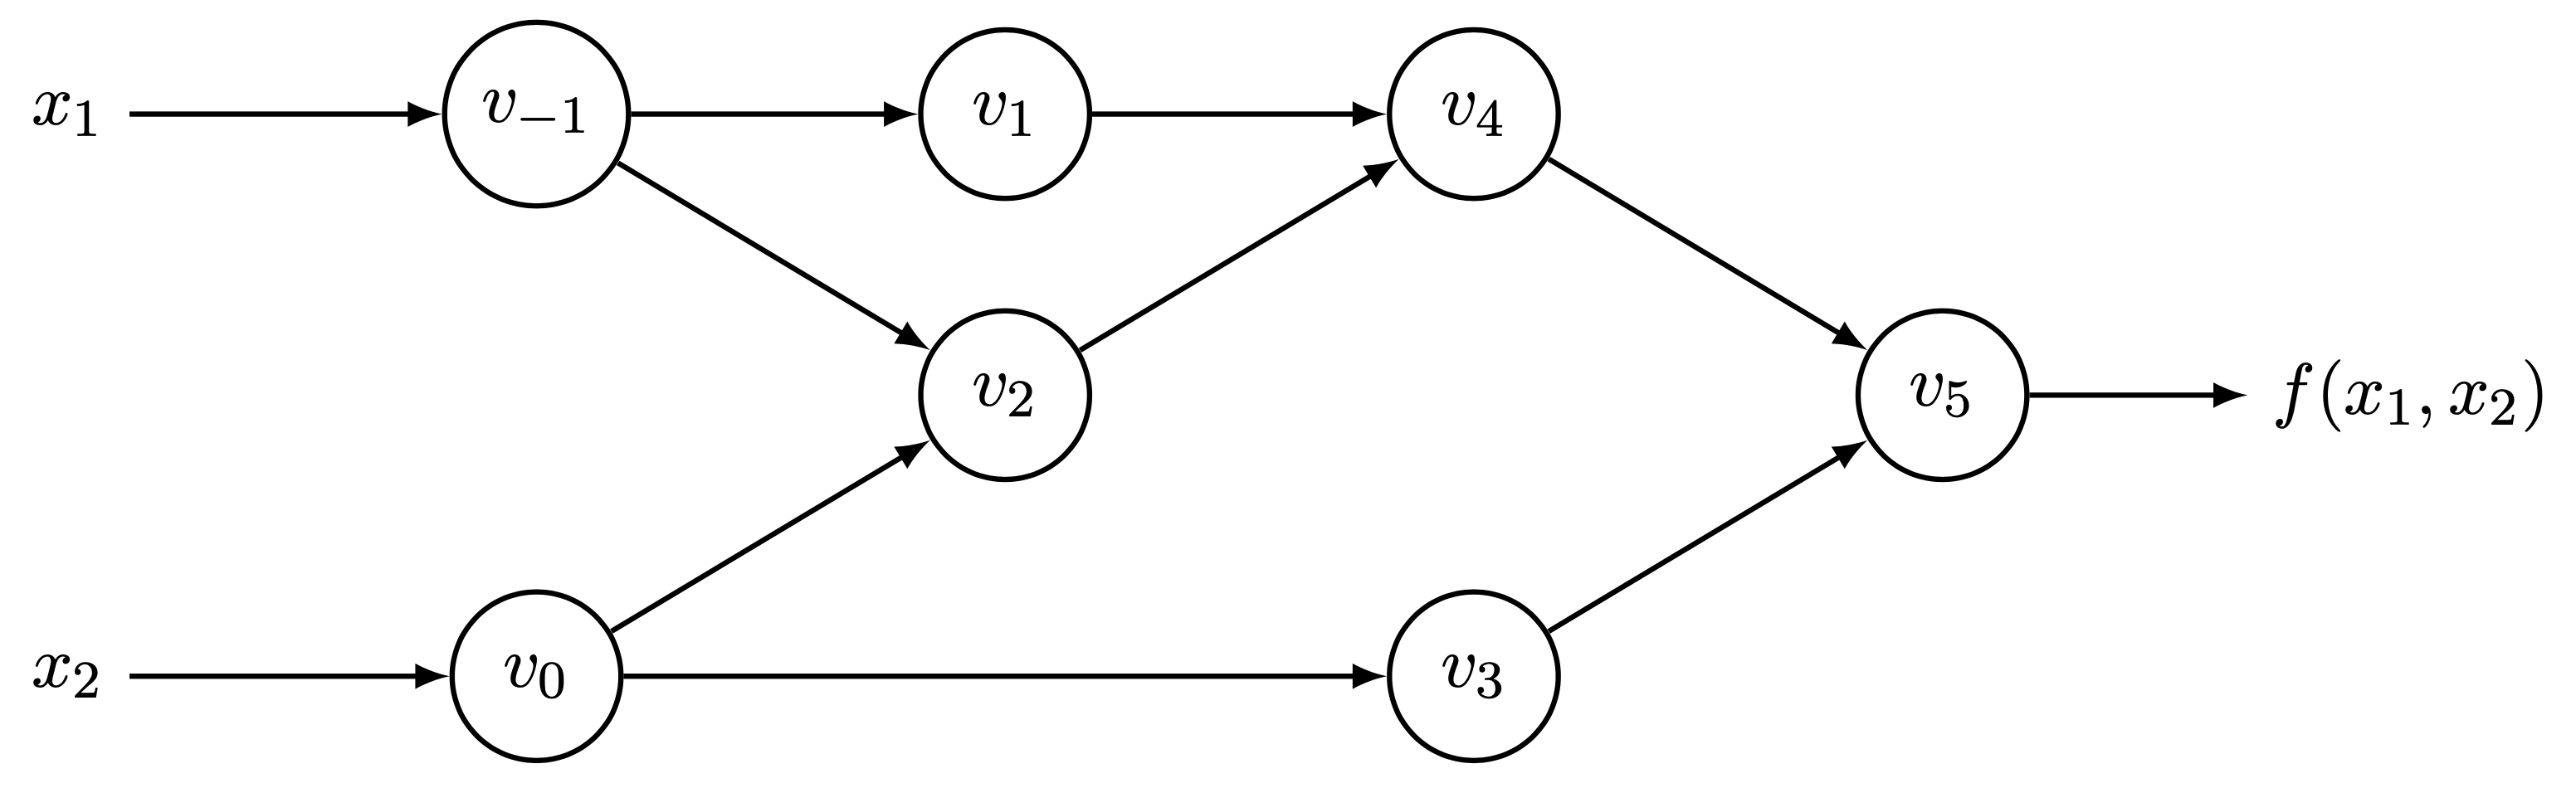
\includegraphics[width = 0.8\hsize]{./figures-autodiff/comp-graph.png}
  \end{figure}
\vspace{-0.3cm}
  \begin{figure}
    \centering
    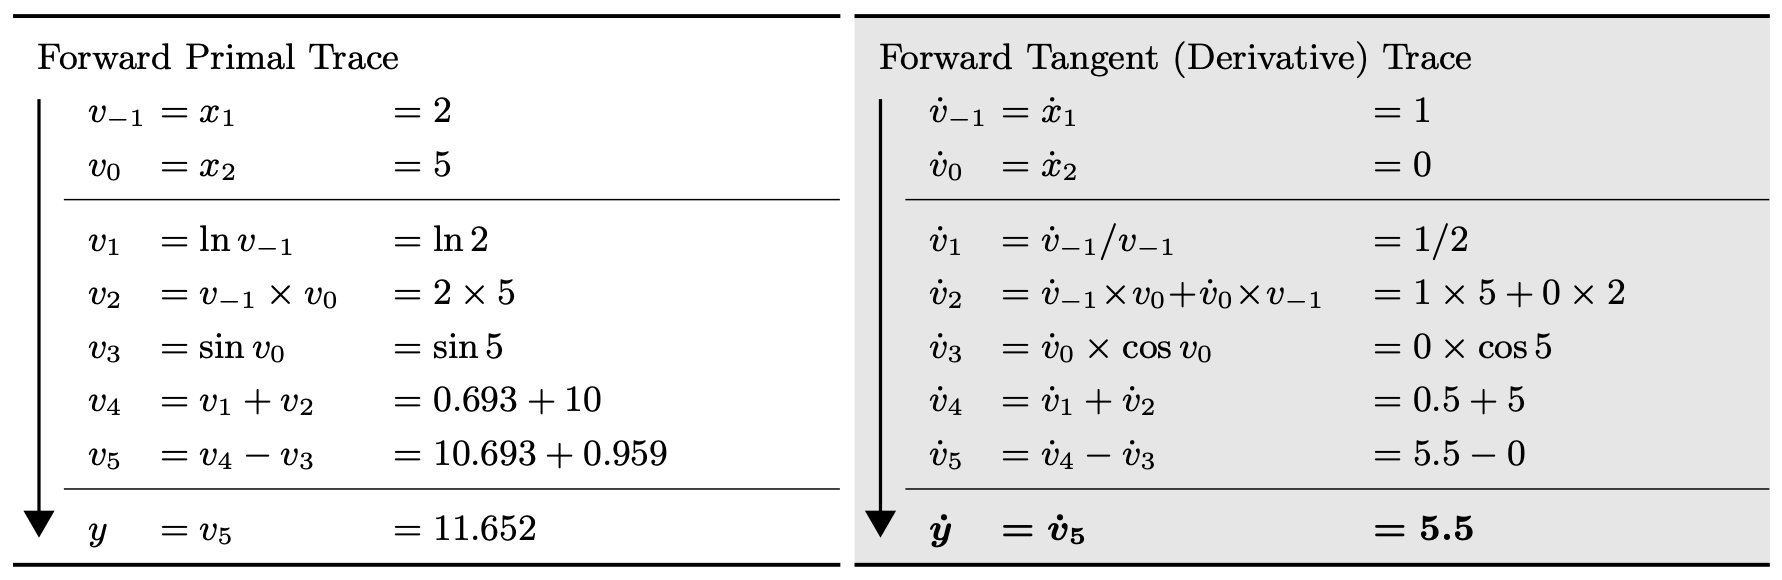
\includegraphics[width = 1.0\hsize]{./figures-autodiff/fwd-trace.png}
  \end{figure}
\end{frame}



\begin{frame}{Things to notice}
\begin{itemize}
\item For each intermediate function $v_j(\{v_k\}_{k\in \mathrm{inputs(j)}})$, you need to implement the equation \cref{eq:fwd}.\pause
\item \emph{All} algorithms are composed of simple functions ($+, *, \mathrm{pow}, \dots$). \pause
\end{itemize}
\begin{center}
\Large You can differentiate anything you implement!
\end{center}\pause

\begin{itemize}
\item $v_j$ and $x_i$ can be vectors: the vector chain rule holds!\pause
\item Implementation can take advantage of any sparsity in $\partial v_j / \partial v_k$. \pause
\end{itemize}
\begin{center}
\Large The procedure above is efficient for vector inputs too!
\end{center}
\end{frame}


\begin{frame}{Forward mode: Computational complexity}
Remember the key equation:
\begin{align}
\pderiv[v_j]{x_i} = \sum_{k \in \mathrm{inputs}(i)} \pderiv[v_j]{v_k}\pderiv[v_k]{x_i}
\end{align}

Consider the scalar case (remember, vector funcs are a special case): \pause
\begin{itemize}
\item The derivative of all elementary functions has the same cost as the computation itself. E.g.~$+, \times, \sin, \mathrm{pow}, \dots$.\pause
\item Only a constant difference in cost between the deriv and func. \pause
\item $\implies$ same computational complexity. \pause
\item No memory overhead. \pause
\item \emph{However}, \pause cost scales linearly with the number of gradients!
\end{itemize}
\end{frame}


\begin{frame}{Fun exercise}
Prove the product rule using forward mode autodiff.
\begin{center}
\emph{Board}
\end{center}
\end{frame}


\section{Reverse Mode Automatic Differentiation}


\begin{frame}{Reverse mode autodiff}
We want to compute the gradient w.r.t.~$x_i$.
\begin{itemize}
\item Traverse the graph to compute the value of all the nodes, \textit{and store them}. \pause
\item Initialise the output node with $\partial \text{out} / \partial v_{\text{final}} = 1$. \pause
\item Traverse the nodes of the graph, indexed by $j$, \textit{backwards}, starting from the output. \pause
\begin{itemize}
\item At the numerically computed values of $v_j$, compute the numerical value of
\begin{align}
\pderiv[\text{out}]{v_j} = \sum_{k \in \mathrm{outputs}(j)} \pderiv[\text{out}]{v_k}\pderiv[v_k]{v_j} \label{eq:bck}
\end{align}
\end{itemize} \pause
\item We end up with $\partial\mathrm{out} / \partial x_i$. \pause
\end{itemize}

\vspace{0.3cm}

Repeat for all $i$ to find all gradients.
\end{frame}


\begin{frame}{Reverse mode Autodiff: Example}
\vspace{-0.5cm}
  Computational graph for $f(x_1, x_2) = \ln(x_1) + x_1x_2 - \sin(x_2)$
  \begin{figure}
    \centering
    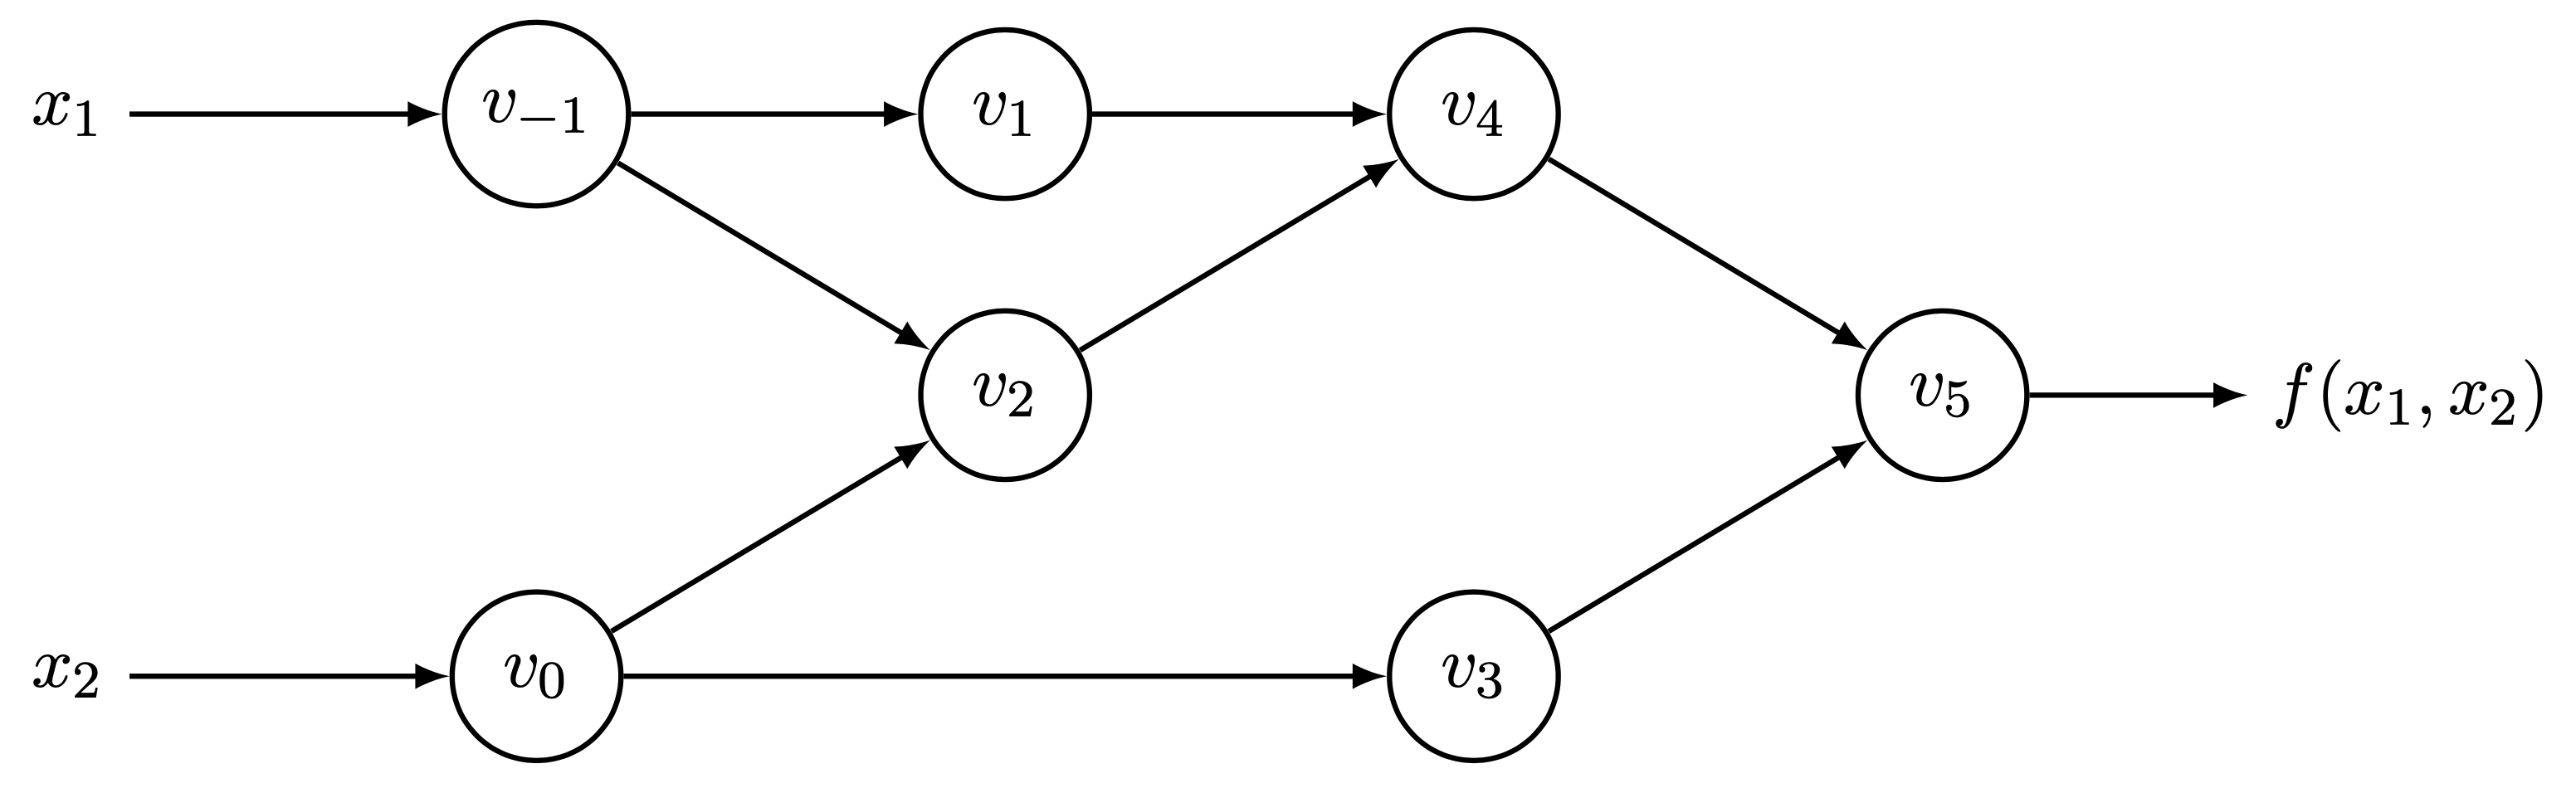
\includegraphics[width = 0.7\hsize]{./figures-autodiff/comp-graph.png}
  \end{figure}
\vspace{-0.4cm}
  \begin{figure}
    \centering
    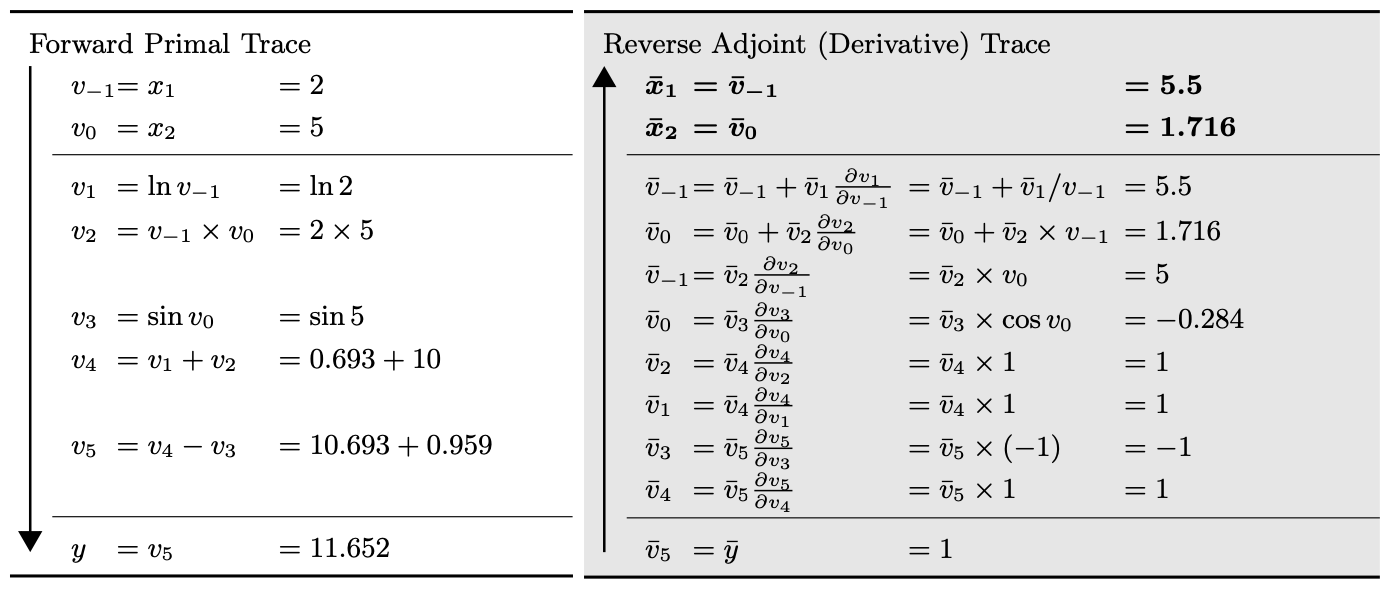
\includegraphics[width = 1.0\hsize]{./figures-autodiff/bck-trace.png}
  \end{figure}
\end{frame}

\begin{frame}{Things to notice (again)}
\begin{itemize}
\item For each intermediate function $v_j(\{v_k\}_{k\in \mathrm{inputs(j)}})$, you need to implement the equation \cref{eq:bck}.\pause
\item \emph{All} algorithms are composed of simple functions ($+, *, \mathrm{pow}, \dots$). \pause
\end{itemize}
\begin{center}
\Large You can differentiate anything you implement!
\end{center}\pause

\begin{itemize}
\item $v_j$ and $x_i$ can be vectors: the vector chain rule holds!\pause
\item Implementation can take advantage of any sparsity in $\partial v_j / \partial v_k$. \pause
\end{itemize}
\begin{center}
\Large The procedure above is efficient for vector inputs too!
\end{center}
\end{frame}


\begin{frame}{Reverse mode: Computational complexity}
Remember the key equation:
\begin{align}
\pderiv[\text{out}]{v_j} = \sum_{k \in \mathrm{outputs}(j)} \pderiv[\text{out}]{v_k}\pderiv[v_k]{v_j}
\end{align}

Consider the scalar case (remember, vector funcs are a special case): \pause
\begin{itemize}
\item The derivative of all elementary functions has the same cost as the computation itself. E.g.~$+, \times, \sin, \mathrm{pow}, \dots$.\pause
\item Only a constant difference in cost between the deriv and func. \pause
\item $\implies$ same computational complexity. \pause
\item Need to store \emph{all} intermediate results (or recompute). \pause
\item \emph{However}, \pause cost of computing all derivatives is same as fwd pass.
\end{itemize}
\end{frame}



\section{Backpropagation in Neural Networks}


%%%%%%%%%%%%%%%%%%%%%%%%%%%%%%%%%%%%%%%%%

\begin{frame}
  \frametitle{Gradients of a Single-Layer Neural Network}
  \begin{figure}
    \centering
    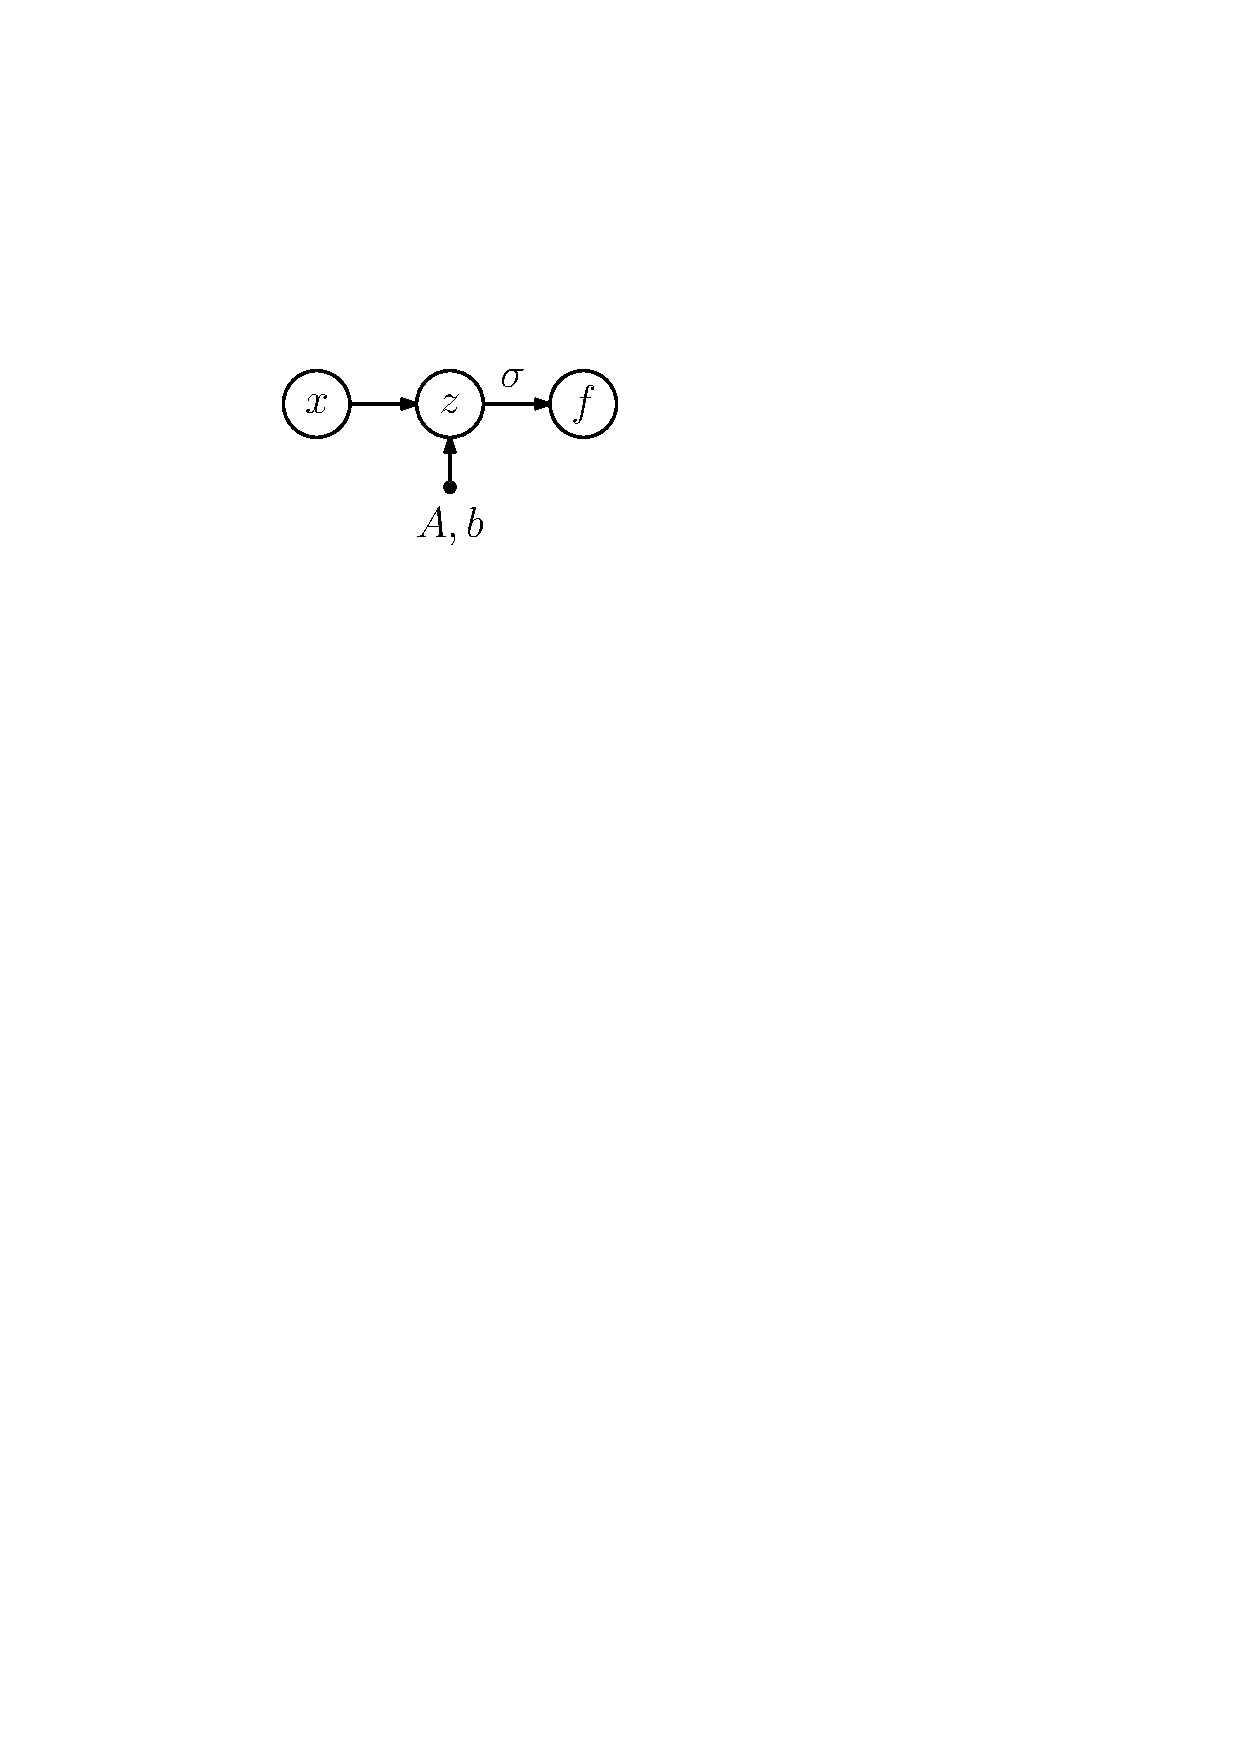
\includegraphics[width = 0.3\hsize]{./figures-backprop/network_z}
  \end{figure}
  
  \begin{align*}
    \vec f &= \tanh(\underbrace{\mat A \vec x + \vec b}_{=:\vec z\in\R^M}) \in\R^M,\quad \vec x \in\R^N, \mat A \in\R^{M\times N}, \vec b\in\R^M
  \end{align*}

\end{frame}

%%%%%%%%%%%%%%%%%%%%%%%%%%%%%%%%%%%%%%%%%
\begin{frame}
  \frametitle{Gradients of a Single-Layer Neural Network}
  
  \begin{align*}
    \vec f &= \tanh(\underbrace{\mat A \vec x + \vec b}_{=:\vec z\in\R^M}) \in\R^M,\quad \vec x \in\R^N, \mat A \in\R^{M\times N}, \vec b\in\R^M\\
    \visible<1->{\frac{\partial \vec f}{\partial\vec b} &=} 
    \visible<2->{\blue{\underbrace{\frac{\partial \vec
    f}{\partial\vec z}}_{{M\times M}}} 
     \red{\underbrace{\frac{\partial \vec z}{\partial \vec b}}_{{M\times M}}} \in\R^{M\times M}}
    \visible<7->{\qquad\qquad\qquad \frac{\partial \vec f}{\partial\mat b}[i,j] = \sum_{l=1}^M \frac{\partial \vec f}{\partial\vec z}[i,l] \frac{\partial\vec z}{\partial \vec b}[l,j]}
    \\
    \visible<1->{\frac{\partial \vec f}{\partial \mat A} &=} 		
    \visible<3->{\blue{\underbrace{\frac{\partial \vec
    f}{\partial\vec z}}_{{M\times M}}} \orange{\underbrace{\frac{\partial
    \vec z}{\partial \mat A}}_{{M\times (M\times N)}}}  \in\R^{M\times (M\times N)}
    \qquad}
    \visible<8->{\frac{\partial \vec f}{\partial\mat A}[i,j,k] = \sum_{l=1}^M \frac{\partial \vec f}{\partial\vec z}[i,l] \frac{\partial\vec z}{\partial \mat A}[l,j,k]}
  \end{align*}
  \vspace{-5mm}
  \begin{align*}
   \visible<4->{\blue{\frac{\partial\vec f}{\partial\vec z}} =\underbrace{\blue{\diag(1 - \tanh^2(\vec z))}}_{\in\:\R^{M\times M}}}
   \quad
	\visible<5->{\red{\frac{\partial \vec z}{\partial \vec b}} =\underbrace{\red{\mat I}}_{\in\:\R^{M\times M}}}
	\quad
	\visible<6->{\orange{\frac{\partial \vec z}{\partial \mat A}} \quad =\underbrace{\orange{\scriptsize\begin{bmatrix}
	\vec x\T & \cdot & \vec 0\T & \cdot & \vec 0\T  \\
	\cdot & & \cdot & & \cdot  \\
	\vec 0\T & \cdot & \vec x\T & \cdot & \vec 0\T \\
	\cdot & & \cdot & & \cdot \\
	\vec 0\T & \cdot & \vec 0\T & \cdot & \vec x\T 
	\end{bmatrix}}}_{\in\:\R^{M \times (M \times N)}}}
  \end{align*}  
\end{frame}

% %%%%%%%%%%%%%%%%%%%%%%%%%%%%%%%%%%%%%%%%%
% \begin{frame}

% \begin{tt}
%  \green{\small
%  import numpy as np\\
%  def NN(x, A, b):\\[1mm]  
%  \qquad     M, N = A.shape\\
    
%  \qquad     z = A.dot(x) + b\\
%  \qquad     f = np.tanh(z)\\[1mm]
    
%  \qquad     \# partial derivatives\\
%  \qquad     dfdz = 1-f**2\\
    
%  \qquad     dzdx = A\\
%  \qquad     dzdb = np.eye(M)\\
%  \qquad     dzdA = np.zeros((M, M, N))\\
    
%  \qquad     for i in range(M):\\
%  \qquad         \qquad dzdA[i,i,:] = x.T\\[1mm]
     
%  \qquad     \# gradients\\
%  \qquad     dfdx = np.einsum('il, lj', dfdz, dzdx)\\
%  \qquad     dfdb = np.einsum('il, lj', dfdz, dzdb)\\
%  \qquad     dfdA = np.einsum('il, ljk', dfdz, dzdA)\\[1mm]
%  \qquad     return f, dfdA, dfdb, dfdx}
%  \end{tt}
%  \end{frame}
  

%%%%%%%%%%%%%%%%%%%%%%%%%%%%%%%%%%%%%%%%%
\begin{frame}
\frametitle{Putting Things Together}
\begin{itemize}[<+->]
  \item Inputs $\vec x \in \R^N$
  \item Observed outputs $\vec y = f_{\vec \theta}(\vec x) + \vec\epsilon \in \R^M \,, \vec \epsilon \sim\gauss{\vec 0}{\mat\Sigma}$
  \item Train single-layer neural network with  
  \begin{align*}
    f_{\vec \theta}(\vec x) =  \tanh(\vec z(\vx)) \in \R^M\,,
    \quad 
    \vec z = \mat A\vec x + \vec b \in \R^M\,,
    \quad 
    \vec\theta = \{\mat A, \vec b\}
  %  \\
  %  \vec t &= \vec f_L
  \end{align*}
  \item Find $\vec A, \vec b$, such that
    the squared loss
    $$
    L(\vec\theta) = \tfrac{1}{2}\|\vec e\|^2 \in \R\,,
    \quad 
    \vec e = \vec y - \vec f_{\vec \theta}(\vec z) \in \R^M
    $$
    is minimized
  \end{itemize}
\end{frame}

\begin{frame}
\frametitle{Putting Things Together}

Partial derivatives:
    \begin{align*}
      \begin{array}{ll}
        \displaystyle
      \frac{\partial L}{\partial \mat A} &\displaystyle = \redish{\frac{\partial L}{\partial
      \vec e}}\frac{\partial\vec e}{\partial \vec f}\blue{\frac{\partial \vec f}{\partial\vec
        z}}\orange{\frac{\partial \vec z}{\partial \mat A}}\\
        \displaystyle
      \frac{\partial L}{\partial \vec b} &\displaystyle =  \redish{\frac{\partial L}{\partial
      \vec e}}\frac{\partial\vec e}{\partial \vec f}\blue{\frac{\partial \vec f}{\partial\vec
        z}}\red{\frac{\partial \vec z}{\partial \vec b}}
      \end{array}
    \end{align*}
    
    \begin{align*}
    \begin{array}{l}
      \displaystyle                                        	  \redish{\frac{\partial L}{\partial
      \vec e} = \underbrace{\vec e\T}_{\in\:\R^{1\times M}}}
      \qquad
      \frac{\partial \vec e}{\partial
      \vec f} = \underbrace{-\vec I}_{\in\:\R^{M \times M}}
      \qquad
      \blue{\frac{\partial \vec
      f}{\partial \mat z} = \underbrace{\diag(1 - \tanh^2(\vec z))}_{\in\:\R^{M\times M}}}
      \\
      \displaystyle
      \orange{\frac{\partial \vec
      z}{\partial \mat A} =
      \underbrace{\begin{bmatrix}
	\vec x\T & \cdot & \vec 0\T & \cdot & \vec 0\T  \\
	\cdot & & \cdot & & \cdot  \\
	\vec 0\T & \cdot & \vec x\T & \cdot & \vec 0\T \\
	\cdot & & \cdot & & \cdot \\
	\vec 0\T & \cdot & \vec 0\T & \cdot & \vec x\T 
	\end{bmatrix}}_{\in\:\R^{M \times (M \times N)}}}
      \qquad  
      \red{\frac{\partial \vec
      z}{\partial \mat b}  = \underbrace{\vec I}_{\in\:\R^{M \times M}}}
    \end{array}
    \end{align*}
\end{frame}

%\begin{frame}
 
% \frametitle{Gradient descent for neural network optimisation}

% \emph{Goal:} Find the local optimum of loss \(L_{\vec \theta^*} \in \R\) where \({\vec \theta}^* = \{\mat A^*, \vec b^* \}\) \\

% Gradient descent algorithm:
% \begin{enumerate}
% \item Initialise neural network parameters, \({\vec \theta}_0\ = \{\mat A_0, \vec b_0 \}\)
% \item Compute gradient of \(L\) w.r.t. parameters, \(\frac{\partial L}{\partial \vec \theta_0}\) 
% \item Update initial guess \({\vec \theta}_0\) using chain rule:
% \begin{align*}
% {\vec \theta_{i+1}} = {\vec \theta_{i}} + \Delta{{\vec \theta}_i} =  {\vec \theta_{i}} - \gamma (\frac{\partial L}{\partial \vec \theta_i} (\vec \theta_i))\T
% \end{align*}
% \arrow Note: parameter update is the direction of steepest \emph{de}scent
% \end{enumerate}

% \visible<2>{
% \vspace{2mm}
% For suitable step-size \(\gamma\), the sequence \( L_{{\vec \theta}_0}(\vec x) \geq L_{{\vec \theta}_1}(\vec x) \geq \cdots\) converges to a local minimum \(L_{\vec \theta^*}(\vec x)\). }

% \visible<1>{
% 	\vspace{-1.3cm}
% 	\begin{figure}
%     \centering
%     \includegraphics[width=0.45\hsize]{./~figures/graddescent.eps}
%   \end{figure}}



% \end{frame}


%%%%%%%%%%%%%%%%%%%%%%%%%%%%%%
\begin{frame}
  \frametitle{Gradients of a Multi-Layer Neural Network}
\vspace{-8mm}
\begin{equation}
L(\vtheta_1, \vtheta_2,\vtheta_3) = ||\vy - \vec f_{\vtheta_3}(\vec f_{\vtheta_2}(\vec f_{\vtheta_1}(\vx)))||^2
\end{equation}
\vspace{-6mm}
\begin{figure}
    \centering
    %\includegraphics[width = 0.8\hsize]{./~figures/NN_forward}
    \scalebox{0.5}{\tikzstyle{ipe stylesheet} = [
  ipe import,
  even odd rule,
  line join=round,
  line cap=butt,
  ipe pen normal/.style={line width=0.4},
  ipe pen heavier/.style={line width=0.8},
  ipe pen fat/.style={line width=1.2},
  ipe pen ultrafat/.style={line width=2},
  ipe pen normal,
  ipe mark normal/.style={ipe mark scale=3},
  ipe mark large/.style={ipe mark scale=5},
  ipe mark small/.style={ipe mark scale=2},
  ipe mark tiny/.style={ipe mark scale=1.1},
  ipe mark normal,
  /pgf/arrow keys/.cd,
  ipe arrow normal/.style={scale=7},
  ipe arrow large/.style={scale=10},
  ipe arrow small/.style={scale=5},
  ipe arrow tiny/.style={scale=3},
  ipe arrow normal,
  /tikz/.cd,
  ipe arrows, % update arrows
  <->/.tip = ipe normal,
  ipe dash normal/.style={dash pattern=},
  ipe dash dashed/.style={dash pattern=on 4bp off 4bp},
  ipe dash dotted/.style={dash pattern=on 1bp off 3bp},
  ipe dash dash dotted/.style={dash pattern=on 4bp off 2bp on 1bp off 2bp},
  ipe dash dash dot dotted/.style={dash pattern=on 4bp off 2bp on 1bp off 2bp on 1bp off 2bp},
  ipe dash normal,
  ipe node/.append style={font=\normalsize},
  ipe stretch normal/.style={ipe node stretch=1},
  ipe stretch normal,
  ipe opacity 10/.style={opacity=0.1},
  ipe opacity 30/.style={opacity=0.3},
  ipe opacity 50/.style={opacity=0.5},
  ipe opacity 75/.style={opacity=0.75},
  ipe opacity opaque/.style={opacity=1},
  ipe opacity opaque,
]
\definecolor{red}{rgb}{1,0,0}%
\definecolor{green}{rgb}{0,1,0}%
\definecolor{blue}{rgb}{0,0,1}%
\definecolor{yellow}{rgb}{1,1,0}%
\definecolor{orange}{rgb}{1,0.647,0}%
\definecolor{gold}{rgb}{1,0.843,0}%
\definecolor{purple}{rgb}{0.627,0.125,0.941}%
\definecolor{gray}{rgb}{0.745,0.745,0.745}%
\definecolor{brown}{rgb}{0.647,0.165,0.165}%
\definecolor{navy}{rgb}{0,0,0.502}%
\definecolor{pink}{rgb}{1,0.753,0.796}%
\definecolor{seagreen}{rgb}{0.18,0.545,0.341}%
\definecolor{turquoise}{rgb}{0.251,0.878,0.816}%
\definecolor{violet}{rgb}{0.933,0.51,0.933}%
\definecolor{darkblue}{rgb}{0,0,0.545}%
\definecolor{darkcyan}{rgb}{0,0.545,0.545}%
\definecolor{darkgray}{rgb}{0.663,0.663,0.663}%
\definecolor{darkgreen}{rgb}{0,0.392,0}%
\definecolor{darkmagenta}{rgb}{0.545,0,0.545}%
\definecolor{darkorange}{rgb}{1,0.549,0}%
\definecolor{darkred}{rgb}{0.545,0,0}%
\definecolor{lightblue}{rgb}{0.678,0.847,0.902}%
\definecolor{lightcyan}{rgb}{0.878,1,1}%
\definecolor{lightgray}{rgb}{0.827,0.827,0.827}%
\definecolor{lightgreen}{rgb}{0.565,0.933,0.565}%%
\definecolor{lightyellow}{rgb}{1,1,0.878}%
\definecolor{black}{rgb}{0,0,0}%
\definecolor{white}{rgb}{1,1,1}%
\begin{tikzpicture}[ipe stylesheet]
  \draw[ipe pen fat]
    (144, 768) rectangle (160, 704);
  \draw[ipe pen fat]
    (256, 768) rectangle (272, 704);
  \draw[ipe pen fat]
    (432, 768) rectangle (448, 704);
  \draw[ipe pen fat]
    (96, 736) circle[radius=16];
  \draw[ipe pen fat]
    (496, 736) circle[radius=16];
  \draw[ipe pen fat, ->]
    (112, 736)
     -- (144, 736);
  \draw[ipe pen fat, ipe dash dashed, ->]
    (272, 736)
     -- (320, 736);
  \draw[ipe pen fat, ->]
    (448, 736)
     -- (480, 736);
  \node[ipe node, font=\Large]
     at (91.741, 732.812) {$\vec{x}$};
  \node[ipe node, font=\Large]
     at (488.698, 732.093) {$\vec{f}_K$};
  \node[ipe node, font=\Large]
     at (135, 664) {$\vec{A}_0, \vec{b}_0$};
  \node[ipe node, font=\Large]
     at (408, 664) {$\vec{A}_{K}, \vec{b}_{K}$};
  \draw[ipe pen fat]
    (560, 736) circle[radius=16];
  \draw[ipe pen fat, ->]
    (512, 736)
     -- (544, 736);
  \node[ipe node, font=\Large]
     at (555.221, 731.099) {$L$};
  \draw[ipe pen fat]
    (320, 768) rectangle (336, 704);
  \draw[ipe pen fat]
    (384, 736) circle[radius=16];
  \draw[ipe pen fat, ->]
    (336, 736)
     -- (368, 736);
  \node[ipe node, font=\Large]
     at (371, 732.508) {$\vec{f}_{K-1}$};
  \draw[ipe pen fat, ->]
    (400, 736)
     -- (432, 736);
  \node[ipe node, font=\Large]
     at (297, 664) {$\vec{A}_{K-1}, \vec{b}_{K-1}$};
  \draw[ipe pen fat, ->]
    (152, 680)
     -- (152, 704);
  \draw[ipe pen fat, ->]
    (264, 680)
     -- (264, 704);
  \draw[ipe pen fat, ->]
    (328, 680)
     -- (328, 704);
  \draw[ipe pen fat, ->]
    (440, 680)
     -- (440, 704);
  \draw[ipe pen fat]
    (208, 736) circle[radius=16];
  \draw[ipe pen fat, ->]
    (160, 736)
     -- (192, 736);
  \node[ipe node, font=\Large]
     at (202.794, 732.093) {$\vec{f}_1$};
  \draw[ipe pen fat, ->]
    (224, 736)
     -- (256, 736);
  \node[ipe node, font=\Large]
     at (247, 664) {$\vec{A}_1, \vec{b}_1$};
\end{tikzpicture}

%%% Local Variables:
%%% mode: latex
%%% TeX-master: "../mml-book"
%%% End:
}
  \end{figure}
  
  \begin{itemize}
  \item Inputs $\vec x$, observed outputs $\vec y$
  \item Train multi-layer neural network with  
  \begin{align*}
    \vec f_0 &= \vec x\\
    \vec f_i &= \sigma_i(\mat A_{i-1}\vec f_{i-1} + \vec b_{i-1})\,,
               \quad i = 1,\dotsc, K
  \end{align*}
  \vspace{-5mm}
  \pause
  \item Find $\vec A_j, \vec b_j$ for $j = 0,\dotsc, K-1$, such that
    the squared loss
    $$
    L(\vec\theta) = \|\vec y - \vec f_{K,\vec \theta}( \vec x)\|^2
    $$
    is minimized, where $
      \vec\theta = \{\mat A_j, \vec b_j\}\,,\quad j = 0, \dotsc, K-1
    $
  \end{itemize}

  
  
\end{frame}


%%%%%%%%%%%%%%%%%%%%%%%%%%%%%%%%%%%%%%%%%
\begin{frame}
  \frametitle{Gradients of a Multi-Layer Neural Network}
\vspace{-8mm}
\begin{equation}
L(\vtheta_1, \vtheta_2,\vtheta_3) = ||\vy - \vec f_{\vtheta_3}(\vec f_{\vtheta_2}(\vec f_{\vtheta_1}(\vx)))||^2
\end{equation}
\vspace{-6mm}
  \onslide*<1>{
  \begin{figure}
    \centering
    % \includegraphics[width = 0.7\hsize]{./~figures/NN1}
     \scalebox{0.5}{\tikzstyle{ipe stylesheet} = [
  ipe import,
  even odd rule,
  line join=round,
  line cap=butt,
  ipe pen normal/.style={line width=0.4},
  ipe pen heavier/.style={line width=0.8},
  ipe pen fat/.style={line width=1.2},
  ipe pen ultrafat/.style={line width=2},
  ipe pen normal,
  ipe mark normal/.style={ipe mark scale=3},
  ipe mark large/.style={ipe mark scale=5},
  ipe mark small/.style={ipe mark scale=2},
  ipe mark tiny/.style={ipe mark scale=1.1},
  ipe mark normal,
  /pgf/arrow keys/.cd,
  ipe arrow normal/.style={scale=7},
  ipe arrow large/.style={scale=10},
  ipe arrow small/.style={scale=5},
  ipe arrow tiny/.style={scale=3},
  ipe arrow normal,
  /tikz/.cd,
  ipe arrows, % update arrows
  <->/.tip = ipe normal,
  ipe dash normal/.style={dash pattern=},
  ipe dash dashed/.style={dash pattern=on 4bp off 4bp},
  ipe dash dotted/.style={dash pattern=on 1bp off 3bp},
  ipe dash dash dotted/.style={dash pattern=on 4bp off 2bp on 1bp off 2bp},
  ipe dash dash dot dotted/.style={dash pattern=on 4bp off 2bp on 1bp off 2bp on 1bp off 2bp},
  ipe dash normal,
  ipe node/.append style={font=\normalsize},
  ipe stretch normal/.style={ipe node stretch=1},
  ipe stretch normal,
  ipe opacity 10/.style={opacity=0.1},
  ipe opacity 30/.style={opacity=0.3},
  ipe opacity 50/.style={opacity=0.5},
  ipe opacity 75/.style={opacity=0.75},
  ipe opacity opaque/.style={opacity=1},
  ipe opacity opaque,
]
\definecolor{red}{rgb}{1,0,0}%
\definecolor{green}{rgb}{0,1,0}%
\definecolor{blue}{rgb}{0,0,1}%
\definecolor{yellow}{rgb}{1,1,0}%
\definecolor{orange}{rgb}{1,0.647,0}%
\definecolor{gold}{rgb}{1,0.843,0}%
\definecolor{purple}{rgb}{0.627,0.125,0.941}%
\definecolor{gray}{rgb}{0.745,0.745,0.745}%
\definecolor{brown}{rgb}{0.647,0.165,0.165}%
\definecolor{navy}{rgb}{0,0,0.502}%
\definecolor{pink}{rgb}{1,0.753,0.796}%
\definecolor{seagreen}{rgb}{0.18,0.545,0.341}%
\definecolor{turquoise}{rgb}{0.251,0.878,0.816}%
\definecolor{violet}{rgb}{0.933,0.51,0.933}%
\definecolor{darkblue}{rgb}{0,0,0.545}%
\definecolor{darkcyan}{rgb}{0,0.545,0.545}%
\definecolor{darkgray}{rgb}{0.663,0.663,0.663}%
\definecolor{darkgreen}{rgb}{0,0.392,0}%
\definecolor{darkmagenta}{rgb}{0.545,0,0.545}%
\definecolor{darkorange}{rgb}{1,0.549,0}%
\definecolor{darkred}{rgb}{0.545,0,0}%
\definecolor{lightblue}{rgb}{0.678,0.847,0.902}%
\definecolor{lightcyan}{rgb}{0.878,1,1}%
\definecolor{lightgray}{rgb}{0.827,0.827,0.827}%
\definecolor{lightgreen}{rgb}{0.565,0.933,0.565}%%
\definecolor{lightyellow}{rgb}{1,1,0.878}%
\definecolor{black}{rgb}{0,0,0}%
\definecolor{white}{rgb}{1,1,1}%
\begin{tikzpicture}[ipe stylesheet]
  \draw[ipe pen fat, white]
    (144, 768) rectangle (160, 704);
  \draw[ipe pen fat, white]
    (256, 768) rectangle (272, 704);
  \draw[ipe pen fat]
    (432, 768) rectangle (448, 704);
  \draw[white, ipe pen fat]
    (96, 736) circle[radius=16];
  \draw[ipe pen fat]
    (496, 736) circle[radius=16];
  \draw[white, ipe pen fat, <-]
    (112, 736)
     -- (144, 736);
  \draw[white, ipe pen fat, ipe dash dashed, <-]
    (272, 736)
     -- (320, 736);
  \draw[red, ipe pen fat, <-]
    (448, 736)
     -- (480, 736);
  \node[ipe node, font=\Large, text=white]
     at (91.741, 732.812) {$\vec{x}$};
  \node[ipe node, font=\Large]
     at (488.698, 734) {$\vec{f}_K$};
  \node[ipe node, font=\Large, text=white]
     at (135, 664) {$\vec{A}_1, \vec{b}_1$};
  \node[ipe node, font=\Large]
     at (408, 664) {$\vec{A}_{K}, \vec{b}_{K}$};
  \draw[ipe pen fat]
    (560, 736) circle[radius=16];
  \draw[red, ipe pen fat, <-]
    (512, 736)
     -- (544, 736);
  \node[ipe node, font=\Large]
     at (555.221, 731.099) {$L$};
  \draw[white, ipe pen fat]
    (320, 768) rectangle (336, 704);
  \draw[white, ipe pen fat]
    (384, 736) circle[radius=16];
  \draw[white, ipe pen fat, <-]
    (336, 736)
     -- (368, 736);
  \node[ipe node, font=\Large, text=white]
     at (371, 734) {$\vec{f}_{K-1}$};
  \draw[white, ipe pen fat, <-]
    (400, 736)
     -- (432, 736);
  \node[ipe node, font=\Large, text=white]
     at (297, 664) {$\vec{A}_{K-1}, \vec{b}_{K-1}$};
  \draw[white, ipe pen fat, ->]
    (152, 680)
     -- (152, 704);
  \draw[white, ipe pen fat, ->]
    (264, 680)
     -- (264, 704);
  \draw[white, ipe pen fat, ->]
    (328, 680)
     -- (328, 704);
  \draw[ipe pen fat, ->]
    (440, 680)
     -- (440, 704);
  \draw[white, ipe pen fat]
    (208, 736) circle[radius=16];
  \draw[white, ipe pen fat, <-]
    (160, 736)
     -- (192, 736);
  \node[ipe node, font=\Large, text=white]
     at (202.794, 734) {$\vec{f}_1$};
  \draw[white, ipe pen fat, <-]
    (224, 736)
     -- (256, 736);
  \node[ipe node, font=\Large, text=white]
     at (247, 664) {$\vec{A}_2, \vec{b}_2$};
\end{tikzpicture}


%%% Local Variables:
%%% mode: latex
%%% TeX-master: "../lecture_vector_calculus"
%%% End:
}
  \end{figure}
}
\onslide*<2>{
  \begin{figure}
    \centering
%    \includegraphics[width = 0.7\hsize]{./~figures/NN2}
    \scalebox{0.5}{\tikzstyle{ipe stylesheet} = [
  ipe import,
  even odd rule,
  line join=round,
  line cap=butt,
  ipe pen normal/.style={line width=0.4},
  ipe pen heavier/.style={line width=0.8},
  ipe pen fat/.style={line width=1.2},
  ipe pen ultrafat/.style={line width=2},
  ipe pen normal,
  ipe mark normal/.style={ipe mark scale=3},
  ipe mark large/.style={ipe mark scale=5},
  ipe mark small/.style={ipe mark scale=2},
  ipe mark tiny/.style={ipe mark scale=1.1},
  ipe mark normal,
  /pgf/arrow keys/.cd,
  ipe arrow normal/.style={scale=7},
  ipe arrow large/.style={scale=10},
  ipe arrow small/.style={scale=5},
  ipe arrow tiny/.style={scale=3},
  ipe arrow normal,
  /tikz/.cd,
  ipe arrows, % update arrows
  <->/.tip = ipe normal,
  ipe dash normal/.style={dash pattern=},
  ipe dash dashed/.style={dash pattern=on 4bp off 4bp},
  ipe dash dotted/.style={dash pattern=on 1bp off 3bp},
  ipe dash dash dotted/.style={dash pattern=on 4bp off 2bp on 1bp off 2bp},
  ipe dash dash dot dotted/.style={dash pattern=on 4bp off 2bp on 1bp off 2bp on 1bp off 2bp},
  ipe dash normal,
  ipe node/.append style={font=\normalsize},
  ipe stretch normal/.style={ipe node stretch=1},
  ipe stretch normal,
  ipe opacity 10/.style={opacity=0.1},
  ipe opacity 30/.style={opacity=0.3},
  ipe opacity 50/.style={opacity=0.5},
  ipe opacity 75/.style={opacity=0.75},
  ipe opacity opaque/.style={opacity=1},
  ipe opacity opaque,
]
\definecolor{red}{rgb}{1,0,0}%
\definecolor{green}{rgb}{0,1,0}%
\definecolor{blue}{rgb}{0,0,1}%
\definecolor{yellow}{rgb}{1,1,0}%
\definecolor{orange}{rgb}{1,0.647,0}%
\definecolor{gold}{rgb}{1,0.843,0}%
\definecolor{purple}{rgb}{0.627,0.125,0.941}%
\definecolor{gray}{rgb}{0.745,0.745,0.745}%
\definecolor{brown}{rgb}{0.647,0.165,0.165}%
\definecolor{navy}{rgb}{0,0,0.502}%
\definecolor{pink}{rgb}{1,0.753,0.796}%
\definecolor{seagreen}{rgb}{0.18,0.545,0.341}%
\definecolor{turquoise}{rgb}{0.251,0.878,0.816}%
\definecolor{violet}{rgb}{0.933,0.51,0.933}%
\definecolor{darkblue}{rgb}{0,0,0.545}%
\definecolor{darkcyan}{rgb}{0,0.545,0.545}%
\definecolor{darkgray}{rgb}{0.663,0.663,0.663}%
\definecolor{darkgreen}{rgb}{0,0.392,0}%
\definecolor{darkmagenta}{rgb}{0.545,0,0.545}%
\definecolor{darkorange}{rgb}{1,0.549,0}%
\definecolor{darkred}{rgb}{0.545,0,0}%
\definecolor{lightblue}{rgb}{0.678,0.847,0.902}%
\definecolor{lightcyan}{rgb}{0.878,1,1}%
\definecolor{lightgray}{rgb}{0.827,0.827,0.827}%
\definecolor{lightgreen}{rgb}{0.565,0.933,0.565}%%
\definecolor{lightyellow}{rgb}{1,1,0.878}%
\definecolor{black}{rgb}{0,0,0}%
\definecolor{white}{rgb}{1,1,1}%
\begin{tikzpicture}[ipe stylesheet]
  \draw[ipe pen fat, white]
    (144, 768) rectangle (160, 704);
  \draw[ipe pen fat, white]
    (256, 768) rectangle (272, 704);
  \draw[ipe pen fat]
    (432, 768) rectangle (448, 704);
  \draw[white, ipe pen fat]
    (96, 736) circle[radius=16];
  \draw[ipe pen fat]
    (496, 736) circle[radius=16];
  \draw[white, ipe pen fat, <-]
    (112, 736)
     -- (144, 736);
  \draw[white, ipe pen fat, ipe dash dashed, <-]
    (272, 736)
     -- (320, 736);
  \draw[red, ipe pen fat, <-]
    (448, 736)
     -- (480, 736);
  \node[ipe node, font=\Large, text=white]
     at (91.741, 732.812) {$\vec{x}$};
  \node[ipe node, font=\Large]
     at (488.698, 734) {$\vec{f}_K$};
  \node[ipe node, font=\Large, text=white]
     at (135, 664) {$\vec{A}_1, \vec{b}_1$};
  \node[ipe node, font=\Large]
     at (408, 664) {$\vec{A}_{K}, \vec{b}_{K}$};
  \draw[ipe pen fat]
    (560, 736) circle[radius=16];
  \draw[red, ipe pen fat, <-]
    (512, 736)
     -- (544, 736);
  \node[ipe node, font=\Large]
     at (555.221, 731.099) {$L$};
  \draw[ipe pen fat]
    (320, 768) rectangle (336, 704);
  \draw[ipe pen fat]
    (384, 736) circle[radius=16];
  \draw[red, ipe pen fat, <-]
    (336, 736)
     -- (368, 736);
  \node[ipe node, font=\Large]
     at (371, 734) {$\vec{f}_{K-1}$};
  \draw[red, ipe pen fat, <-]
    (400, 736)
     -- (432, 736);
  \node[ipe node, font=\Large]
     at (297, 664) {$\vec{A}_{K-1}, \vec{b}_{K-1}$};
  \draw[white, ipe pen fat, ->]
    (152, 680)
     -- (152, 704);
  \draw[white, ipe pen fat, ->]
    (264, 680)
     -- (264, 704);
  \draw[ ipe pen fat, ->]
    (328, 680)
     -- (328, 704);
  \draw[ipe pen fat, ->]
    (440, 680)
     -- (440, 704);
  \draw[white, ipe pen fat]
    (208, 736) circle[radius=16];
  \draw[white, ipe pen fat, <-]
    (160, 736)
     -- (192, 736);
  \node[ipe node, font=\Large, text=white]
     at (202.794, 734) {$\vec{f}_1$};
  \draw[white, ipe pen fat, <-]
    (224, 736)
     -- (256, 736);
  \node[ipe node, font=\Large, text=white]
     at (247, 664) {$\vec{A}_2, \vec{b}_2$};
\end{tikzpicture}



% \begin{tikzpicture}[ipe stylesheet]
%   \draw[white, ipe pen fat]
%     (144, 768) rectangle (160, 704);
%   \draw[white, ipe pen fat]
%     (256, 768) rectangle (272, 704);
%   \draw[ipe pen fat]
%     (432, 768) rectangle (448, 704);
%   \draw[white, ipe pen fat]
%     (96, 736) circle[radius=16];
%   \draw[ipe pen fat]
%     (496, 736) circle[radius=16];
%   \draw[white, ipe pen fat, ->]
%     (112, 736)
%      -- (144, 736);
%   \draw[white, ipe pen fat, ipe dash dashed, ->]
%     (272, 728)
%      -- (320, 728);
%   \draw[ipe pen fat, ->]
%     (448, 728)
%      -- (480, 728);
%   \node[ipe node, font=\Large, text=white]
%      at (92.009, 732.912) {$\vec x$};
%   \node[ipe node, font=\Large]
%      at (488.899, 732.414) {$\vec f_K$};
%   \node[ipe node, font=\Large, text=white]
%      at (135.123, 664) {$\vec A_1, \vec b_1$};
%   \node[ipe node, font=\Large]
%      at (408.594, 664) {$\mat A_{K-1}, \vec b_{K-1}$};
%   \draw[red, ipe pen fat, ->]
%     (480, 744)
%      -- (448, 744);
%   \draw[white, ipe pen fat, ipe dash dashed, ->]
%     (320, 744)
%      -- (272, 744);
%   \draw[ipe pen fat]
%     (560, 736) circle[radius=16];
%   \draw[ipe pen fat, ->]
%     (512, 728)
%      -- (544, 728);
%   \draw[red, ipe pen fat, ->]
%     (544, 744)
%      -- (512, 744);
%   \node[ipe node, font=\Large]
%      at (555.221, 731.099) {$L$};
%   \draw[ipe pen fat]
%     (320, 768) rectangle (336, 704);
%   \draw[ipe pen fat]
%     (384, 736) circle[radius=16];
%   \draw[ipe pen fat, ->]
%     (336, 728)
%      -- (368, 728);
%   \node[ipe node, font=\Large]
%      at (370.534, 732.508) {$\vec f_{K-1}$};
%   \draw[red, ipe pen fat, ->]
%     (368, 744)
%      -- (336, 744);
%   \draw[ipe pen fat, ->]
%     (400, 728)
%      -- (432, 728);
%   \draw[red, ipe pen fat, ->]
%     (432, 744)
%      -- (400, 744);
%   \node[ipe node, font=\Large]
%      at (296.594, 664) {$\mat A_{K-2}, \vec b_{K-2}$};
%   \draw[white, ipe pen fat, ->]
%     (152, 680)
%      -- (152, 704);
%   \draw[white, ipe pen fat, ->]
%     (264, 680)
%      -- (264, 704);
%   \draw[ipe pen fat, ->]
%     (328, 680)
%      -- (328, 704);
%   \draw[ipe pen fat, ->]
%     (440, 680)
%      -- (440, 704);
%   \pic[ipe mark large, white]
%      at (152, 680) {ipe disk};
%   \pic[ipe mark large, white]
%      at (264, 680) {ipe disk};
%   \pic[ipe mark large]
%      at (328, 680) {ipe disk};
%   \pic[ipe mark large]
%      at (440, 680) {ipe disk};
%   \draw[white, ipe pen fat]
%     (208, 736) circle[radius=16];
%   \draw[white, ipe pen fat, ->]
%     (160, 728)
%      -- (192, 728);
%   \node[ipe node, font=\Large, text=white]
%      at (200.899, 732.414) {$f_1$};
%   \draw[white, ipe pen fat, ->]
%     (192, 744)
%      -- (160, 744);
%   \draw[white, ipe pen fat, ->]
%     (224, 728)
%      -- (256, 728);
%   \draw[white, ipe pen fat, ->]
%     (256, 744)
%      -- (224, 744);
%   \node[ipe node, font=\Large, text=white]
%      at (247.123, 664) {$A_2, b_2$};
% \end{tikzpicture}

%%% Local Variables:
%%% mode: latex
%%% TeX-master: "../lecture_vector_calculus"
%%% End:
}
  \end{figure}
}
\onslide*<3->{
 \begin{figure}
   \centering
  \scalebox{0.5}{\tikzstyle{ipe stylesheet} = [
  ipe import,
  even odd rule,
  line join=round,
  line cap=butt,
  ipe pen normal/.style={line width=0.4},
  ipe pen heavier/.style={line width=0.8},
  ipe pen fat/.style={line width=1.2},
  ipe pen ultrafat/.style={line width=2},
  ipe pen normal,
  ipe mark normal/.style={ipe mark scale=3},
  ipe mark large/.style={ipe mark scale=5},
  ipe mark small/.style={ipe mark scale=2},
  ipe mark tiny/.style={ipe mark scale=1.1},
  ipe mark normal,
  /pgf/arrow keys/.cd,
  ipe arrow normal/.style={scale=7},
  ipe arrow large/.style={scale=10},
  ipe arrow small/.style={scale=5},
  ipe arrow tiny/.style={scale=3},
  ipe arrow normal,
  /tikz/.cd,
  ipe arrows, % update arrows
  <->/.tip = ipe normal,
  ipe dash normal/.style={dash pattern=},
  ipe dash dashed/.style={dash pattern=on 4bp off 4bp},
  ipe dash dotted/.style={dash pattern=on 1bp off 3bp},
  ipe dash dash dotted/.style={dash pattern=on 4bp off 2bp on 1bp off 2bp},
  ipe dash dash dot dotted/.style={dash pattern=on 4bp off 2bp on 1bp off 2bp on 1bp off 2bp},
  ipe dash normal,
  ipe node/.append style={font=\normalsize},
  ipe stretch normal/.style={ipe node stretch=1},
  ipe stretch normal,
  ipe opacity 10/.style={opacity=0.1},
  ipe opacity 30/.style={opacity=0.3},
  ipe opacity 50/.style={opacity=0.5},
  ipe opacity 75/.style={opacity=0.75},
  ipe opacity opaque/.style={opacity=1},
  ipe opacity opaque,
]
\definecolor{red}{rgb}{1,0,0}%
\definecolor{black}{rgb}{0,0,0}%
\definecolor{white}{rgb}{1,1,1}%
\begin{tikzpicture}[ipe stylesheet]
  \draw[ipe pen fat]
    (144, 768) rectangle (160, 704);
  \draw[ipe pen fat]
    (256, 768) rectangle (272, 704);
  \draw[ipe pen fat]
    (432, 768) rectangle (448, 704);
  \draw[ipe pen fat]
    (96, 736) circle[radius=16];
  \draw[ipe pen fat]
    (496, 736) circle[radius=16];
  \draw[red, ipe pen fat, <-]
    (112, 736)
     -- (144, 736);
  \draw[red, ipe pen fat, ipe dash dashed, <-]
    (272, 736)
     -- (320, 736);
  \draw[red, ipe pen fat, <-]
    (448, 736)
     -- (480, 736);
  \node[ipe node, font=\Large]
     at (91.741, 734) {$\vec{x}$};
  \node[ipe node, font=\Large]
     at (488.698, 734) {$\vec{f}_K$};
  \node[ipe node, font=\Large]
     at (135, 664) {$\vec{A}_1, \vec{b}_1$};
  \node[ipe node, font=\Large]
     at (408, 664) {$\vec{A}_{K}, \vec{b}_{K}$};
  \draw[ipe pen fat]
    (560, 736) circle[radius=16];
  \draw[red, ipe pen fat, <-]
    (512, 736)
     -- (544, 736);
  \node[ipe node, font=\Large]
     at (555.221, 731.099) {$L$};
  \draw[ipe pen fat]
    (320, 768) rectangle (336, 704);
  \draw[ipe pen fat]
    (384, 736) circle[radius=16];
  \draw[red, ipe pen fat, <-]
    (336, 736)
     -- (368, 736);
  \node[ipe node, font=\Large]
     at (371, 734) {$\vec{f}_{K-1}$};
  \draw[red, ipe pen fat, <-]
    (400, 736)
     -- (432, 736);
  \node[ipe node, font=\Large]
     at (297, 664) {$\vec{A}_{K-1}, \vec{b}_{K-1}$};
  \draw[ipe pen fat, ->]
    (152, 680)
     -- (152, 704);
  \draw[ipe pen fat, ->]
    (264, 680)
     -- (264, 704);
  \draw[ipe pen fat, ->]
    (328, 680)
     -- (328, 704);
  \draw[ipe pen fat, ->]
    (440, 680)
     -- (440, 704);
  \draw[ipe pen fat]
    (208, 736) circle[radius=16];
  \draw[red, ipe pen fat, <-]
    (160, 736)
     -- (192, 736);
  \node[ipe node, font=\Large]
     at (202.794, 734) {$\vec{f}_1$};
  \draw[red, ipe pen fat, <-]
    (224, 736)
     -- (256, 736);
  \node[ipe node, font=\Large]
     at (247, 664) {$\vec{A}_2, \vec{b}_2$};
\end{tikzpicture}

%%% Local Variables:
%%% mode: latex
%%% TeX-master: "../lecture_vector_calculus"
%%% End:
}
 \end{figure}
}
\vspace{-3mm}
  \begin{align*}
 \onslide+<1->{   \frac{\partial L}{\partial\vec\theta_{K}} &= \orange{\frac{\partial L}{\partial \vec f_K}}\blue{\frac{\partial \vec f_K}{\partial \vec\theta_{K}}}\\
}
    \onslide+<2->{    \frac{\partial L}{\partial\vec\theta_{K-1}} &=\orange{\frac{\partial
                                                                    L}{\partial \vec f_K}}
                                                                    \boxed{ \green{\frac{\partial \vec f_K}{\partial
                                                                    \vec f_{K-1}}}
                                                                    \blue{\frac{\partial\vec
                                                                    f_{K-1}}{\partial \vec\theta_{K-1}}}}\\}
    \onslide+<3->{    \frac{\partial L}{\partial\vec\theta_{K-2}} &=\orange{\frac{\partial
                                                                    L}{\partial \vec f_K}}
                                                                    \green{\frac{\partial \vec f_K}{\partial
                                                                    \vec f_{K-1}}} \boxed{\green{\frac{\partial \vec f_{K-1}}{\partial
                                                                    \vec f_{K-2}}}
                                                                    \blue{\frac{\partial\vec
                                                                    f_{K-2}}{\partial \vec\theta_{K-2}}}}\\}
    \onslide+<4->{    \frac{\partial L}{\partial\vec\theta_{i}} &=\orange{\frac{\partial
                                                                  L}{\partial \vec f_K}}
                                                                  \green{\frac{\partial \vec f_K}{\partial
                                                                  \vec f_{K-1}}\cdots}\boxed{\green{\frac{\partial \vec f_{i+1}}{\partial
                                                                  \vec f_{i}}}
                                                                  \blue{\frac{\partial\vec
                                                                  f_{i}}{\partial
                                                                  \vec\theta_{i}}}}
                                                                  }
  \end{align*}
\onslide+<5>{\arrow Intermediate derivatives are stored during the forward pass}

  % \begin{align*}
  %   \frac{\partial \vec f_j}{\partial\vec f_{j-1}} = \mat A_{j-1}
  % \end{align*}
\end{frame}



% %%%%%%%%%%%%%%%%%%%%%%%%%%%%%%%%%%%%%%%%%%%%%%%%%%%%%%
%   \begin{frame}
%     \frametitle{Example: Regression with Neural Networks}

%     \begin{itemize}
%     \item Linear regression with a neural network parametrized by \(\vec \theta, f_{\vec \theta}\):
%       \begin{align*}
%         y &= f_{\vec \theta}(\vec x) + \epsilon\,,\quad \epsilon \sim \gauss{0}{\sigma_\epsilon^2}
%       \end{align*}
%       \pause
%     \item Given inputs $\vec x_n$ and corresponding (noisy)
%       observations $y_n$, $n=1,\dotsc, N$, find parameters
%       $\vec \theta^*$ that minimize the squared loss
%         $$
%         L(\vec\theta) = \sum_{n=1}^N (y_n - f_{\vec \theta}(\vec x_n))^2 =
%         \norm{\vec y - \vec f(\mat X)}^2
%         $$
%   \end{itemize}
    
    
%  \end{frame}




%%% Local Variables:
%%% mode: latex
%%% TeX-master: "lecture_vector_calculus"
%%% End:

% %%%%%%%%%%%%%%%%%%%%%%%%%%%%%%%%%%%%%%%%%%%%%%%%%%%%%%
% \begin{frame}
%   \frametitle{Training Neural Networks as Maximum Likelihood Estimation}
%   \begin{itemize}
%   \item Training a neural network in the above way corresponds to
%     \cemph{maximum likelihood estimation:}
%       \begin{itemize}
%         \item If $\vec y = NN(\vec x, \vec\theta) + \vec\epsilon,
%           \quad \vec\epsilon \sim \gauss{\vec 0}{\mat I}$ then the
%           \cemph{log-likelihood} is
%           $$
%           \log p(\vec y|\vec X, \vec\theta) =
%           -\tfrac{1}{2}\|\vec y - NN(\vec x,
%             \vec\theta)\|^2
%             $$
%             \pause
%           \item Find $\vec\theta^*$ by \cemph{minimizing the negative
%             log-likelihood:}
%             \begin{align*}
%               \vec\theta^* &= \arg\min_{\vec\theta}-\log p(\vec y|\vec
%                              x, \vec\theta) \\
%                            &=  \arg\min_{\vec\theta} \tfrac{1}{2}\|\vec y - NN(\vec x,
%                              \vec\theta)\|^2 \\
%                            &= \arg\min_{\vec\theta}L(\vec\theta)
%             \end{align*}
%           \end{itemize}
%           \pause
%           \item Maximum likelihood estimation can lead to
%             \calert{overfitting} (interpret noise as signal)
%     \end{itemize}
%   \end{frame}

  % %%%%%%%%%%%%%%%%%%%%%%%%%%%%%%%%%%%%%%%%%%%%%%%%%%%%%%
  % \begin{frame}
  %   \frametitle{Example: Linear Regression (1)}

  %   \begin{itemize}
  %   \item Linear regression with a polynomial of order $M$:
  %     \begin{align*}
  %       y &= f(x,\vec\theta) + \epsilon\,,\quad \epsilon \sim \gauss{0}{\sigma_\epsilon^2}\\
  %       f(x,\vec\theta) &= \theta_0 + \theta_1x + \theta_2 x^2 + \cdots + \theta_Mx^M = \sum_{i = 0}^M \theta_ix^i
  %     \end{align*}
  %     \pause
  %     \item Given inputs $x_i$ and corresponding (noisy) observations
  %       $y_i$, $i=1,\dotsc, N$, find parameters $\vec \theta = [\theta_0, \dotsc,
  %       \theta_M]\T$, that minimize the squared loss (equivalently: maximize the likelihood)
  %       $$
  %       L(\vec\theta) = \sum_{i=1}^N (y_i - f(x_i, \vec\theta))^2
  %       $$
  % \end{itemize}
    
    
  % \end{frame}

% %%%%%%%%%%%%%%%%%%%%%%%%%%%%%%%%%%%%%%%%%%%%%%%%%%%%%%
% \begin{frame}
%   \frametitle{Example: Linear Regression (2)}

%   \begin{figure}
%     \centering
%     \includegraphics[width = 0.5\hsize]{./~figures/polynomial16}
%   \end{figure}
%   \pause
%   \begin{itemize}
%   \item Regularization, model selection etc. can address overfitting
%   \item Alternative approach based on integration 
% \end{itemize}

  
% \end{frame}
          


% \nocite{Roberts2013, Krause2008, Deisenroth2015b, Deisenroth2009,Deisenroth2015, Calandra2014,Calandra2015a,
%   Calandra2014b,  Deisenroth2011c,
%   Quinonero-Candela2003a, Rasmussen2006, Sutton1998, Bertsekas2005,
%    Jones1998, Brochu2009, Osborne2009, Bertone2016, Baroukh2014,
%   Deisenroth2012d, Deisenroth2012,Frigola2013,Kocijan2004,Quinonero-Candela2005}





% \begin{frame}[t]{Summary}
%   \begin{center}
%     \scalebox{0.3}{\input{./~figures/gradients_new.tex}}
%         \includegraphics[height = 3cm]{./~figures/polynomial16}\\
%     \scalebox{0.4}{\tikzstyle{ipe stylesheet} = [
  ipe import,
  even odd rule,
  line join=round,
  line cap=butt,
  ipe pen normal/.style={line width=0.4},
  ipe pen heavier/.style={line width=0.8},
  ipe pen fat/.style={line width=1.2},
  ipe pen ultrafat/.style={line width=2},
  ipe pen normal,
  ipe mark normal/.style={ipe mark scale=3},
  ipe mark large/.style={ipe mark scale=5},
  ipe mark small/.style={ipe mark scale=2},
  ipe mark tiny/.style={ipe mark scale=1.1},
  ipe mark normal,
  /pgf/arrow keys/.cd,
  ipe arrow normal/.style={scale=7},
  ipe arrow large/.style={scale=10},
  ipe arrow small/.style={scale=5},
  ipe arrow tiny/.style={scale=3},
  ipe arrow normal,
  /tikz/.cd,
  ipe arrows, % update arrows
  <->/.tip = ipe normal,
  ipe dash normal/.style={dash pattern=},
  ipe dash dashed/.style={dash pattern=on 4bp off 4bp},
  ipe dash dotted/.style={dash pattern=on 1bp off 3bp},
  ipe dash dash dotted/.style={dash pattern=on 4bp off 2bp on 1bp off 2bp},
  ipe dash dash dot dotted/.style={dash pattern=on 4bp off 2bp on 1bp off 2bp on 1bp off 2bp},
  ipe dash normal,
  ipe node/.append style={font=\normalsize},
  ipe stretch normal/.style={ipe node stretch=1},
  ipe stretch normal,
  ipe opacity 10/.style={opacity=0.1},
  ipe opacity 30/.style={opacity=0.3},
  ipe opacity 50/.style={opacity=0.5},
  ipe opacity 75/.style={opacity=0.75},
  ipe opacity opaque/.style={opacity=1},
  ipe opacity opaque,
]
\definecolor{red}{rgb}{1,0,0}%
\definecolor{black}{rgb}{0,0,0}%
\definecolor{white}{rgb}{1,1,1}%
\begin{tikzpicture}[ipe stylesheet]
  \draw[ipe pen fat]
    (144, 768) rectangle (160, 704);
  \draw[ipe pen fat]
    (256, 768) rectangle (272, 704);
  \draw[ipe pen fat]
    (432, 768) rectangle (448, 704);
  \draw[ipe pen fat]
    (96, 736) circle[radius=16];
  \draw[ipe pen fat]
    (496, 736) circle[radius=16];
  \draw[red, ipe pen fat, <-]
    (112, 736)
     -- (144, 736);
  \draw[red, ipe pen fat, ipe dash dashed, <-]
    (272, 736)
     -- (320, 736);
  \draw[red, ipe pen fat, <-]
    (448, 736)
     -- (480, 736);
  \node[ipe node, font=\Large]
     at (91.741, 734) {$\vec{x}$};
  \node[ipe node, font=\Large]
     at (488.698, 734) {$\vec{f}_K$};
  \node[ipe node, font=\Large]
     at (135, 664) {$\vec{A}_1, \vec{b}_1$};
  \node[ipe node, font=\Large]
     at (408, 664) {$\vec{A}_{K}, \vec{b}_{K}$};
  \draw[ipe pen fat]
    (560, 736) circle[radius=16];
  \draw[red, ipe pen fat, <-]
    (512, 736)
     -- (544, 736);
  \node[ipe node, font=\Large]
     at (555.221, 731.099) {$L$};
  \draw[ipe pen fat]
    (320, 768) rectangle (336, 704);
  \draw[ipe pen fat]
    (384, 736) circle[radius=16];
  \draw[red, ipe pen fat, <-]
    (336, 736)
     -- (368, 736);
  \node[ipe node, font=\Large]
     at (371, 734) {$\vec{f}_{K-1}$};
  \draw[red, ipe pen fat, <-]
    (400, 736)
     -- (432, 736);
  \node[ipe node, font=\Large]
     at (297, 664) {$\vec{A}_{K-1}, \vec{b}_{K-1}$};
  \draw[ipe pen fat, ->]
    (152, 680)
     -- (152, 704);
  \draw[ipe pen fat, ->]
    (264, 680)
     -- (264, 704);
  \draw[ipe pen fat, ->]
    (328, 680)
     -- (328, 704);
  \draw[ipe pen fat, ->]
    (440, 680)
     -- (440, 704);
  \draw[ipe pen fat]
    (208, 736) circle[radius=16];
  \draw[red, ipe pen fat, <-]
    (160, 736)
     -- (192, 736);
  \node[ipe node, font=\Large]
     at (202.794, 734) {$\vec{f}_1$};
  \draw[red, ipe pen fat, <-]
    (224, 736)
     -- (256, 736);
  \node[ipe node, font=\Large]
     at (247, 664) {$\vec{A}_2, \vec{b}_2$};
\end{tikzpicture}

%%% Local Variables:
%%% mode: latex
%%% TeX-master: "../lecture_vector_calculus"
%%% End:
}

% \end{center}
% \begin{itemize}
%   \item Vector-valued differentiation
%   \item Chain rule
%   \item Check the dimension of the gradients
%   \end{itemize}
% \end{frame}


\begin{frame}{Summary: Differentiation}
\begin{itemize}
\item Computational graphs
\item Flavours of automatic differentiation
\item Computational cost analysis of automatic differentiation
\item Application: Backpropagation in NNs
\end{itemize} \pause

\vspace{0.5cm}
If you have a spare 1.5 hours, and want to see how \emph{minimal} an implementation of this can be, I \emph{highly} recommend Conal Elliott's talk on \textit{The Simple Essence of Automatic Differentiation}: 
https://www.youtube.com/watch?v=ne99laPUxN4
\end{frame}

% %%%%%%%%%%%%%%%%%%%%%%%%%%%%%%%%%%%%%%%%%
% % REFERENCES
% %%%%%%%%%%%%%%%%%%%%%%%%%%%%%%%%%%%%%%%%%
\begin{frame}[t,allowframebreaks]
\frametitle{References}
\linespread{1.0}
\tiny
\bibliographystyle{plainnat}
\bibliography{../includes/ref.bib}
\end{frame}


\end{document}